%%%%%%%%%%%%%%%%%%%%%%%%%%%%%%%%%%%%%%%%%%%%%%%%%%%%%%%%%%%%%%%%%%%%%%%%
%                                                                      %
%     File: Thesis_Results.tex                                         %
%     Tex Master: Thesis.tex                                           %
%                                                                      %
%     Author: Andre C. Marta                                           %
%     Last modified :  4 Mar 2024                                      %
%                                                                      %
%%%%%%%%%%%%%%%%%%%%%%%%%%%%%%%%%%%%%%%%%%%%%%%%%%%%%%%%%%%%%%%%%%%%%%%%

\chapter{iQAQE Schemes and Results}
\label{chapter:Schemes_and_Results}

% Before I start mindlessly dumping things here, I should re-read everything on the logbook, so I have a better idea of what I want to say. Also, I shouldn't include all of what is said there, probably. I think I'll just write all that I want to say and, if need be, I'll cut some things in the end, once I'm re-reading the ENTIRE thing, again.

% Insert your chapter material here. - In this chapter, we should present all the many schemes that we've come up with, and the results of the numerical simulations of these schemes. We should also compare the results of the different schemes, and discuss the potential of each one. We should also mention the importance of the results and the potential applications of the schemes. This will, surely, be the largest chapter of the thesis.

% Here, I should present each realization of iQAQE, theoretically, as well as the results of the numerical simulations of each realization. I should also mention that this work is, essentially, a collection/compilation of different schemes/ideas, all inspired by the base-iQAQE algorithm, described above. As such, some schemes will appear disconnected from others, but they all serve the same purpose, ultimately. (This is how I should justify the existence of so many schemes, and the lack of a clear connection between them. Also, this is how one should look at this.)

% I might re-order these a little.


In this chapter, we present the various \acrshort{iqaqe} schemes we have developed and the results of their numerical simulations. These schemes explore different combinations of qubit numbers, list cardinalities, basis state mappings, and circuit layers. Each scheme features a unique mapping, resulting in distinct outcomes and properties. We compare these results and discuss the potential of each scheme. This chapter is essentially a collection of various ideas, all built upon the \acrshort{iqaqe} Framework described in Chapter \ref{chapter:Base Algorithm}. While some schemes may seem disconnected, they all contribute to the overall goal, justifying their inclusion.

At times, our work diverged from \acrshort{iqaqe}, leading us to explore other ideas for MaxCut algorithms. Although these ideas originated from our work on \acrshort{iqaqe}, they are distinct enough to warrant their own chapter. These will be presented in the next chapter (Chapter \ref{chapter:Exploratory_Ideas}).

From here onwards, unless explicitly stated otherwise, all \acrshort{vqa}\textcolor{gray}{s} are being tested on the following $8$-node graph, whose optimal cut is $10$ (Figure \ref{fig:8_node_graph}). This graph is one of the benchmarks used in \cite{tenecohen2023variational}, which is why we employ it here. Additionally, its small size allows for reasonably quick simulations on my personal computer, which is a significant advantage.

\begin{figure}[H]
    \centering
    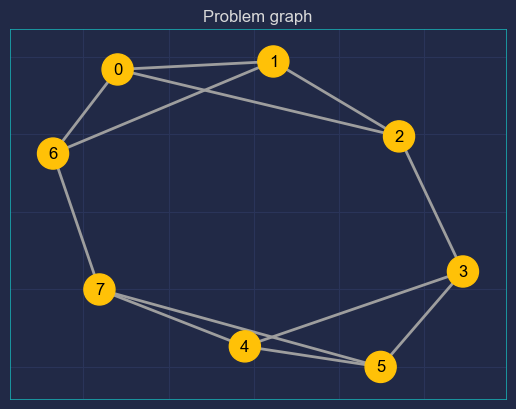
\includegraphics[width=0.55\textwidth]{Figures/Chapter_5/problem_graph.png}
    \caption{Considered $8$-node graph instance. The optimal cut ($10$) was found through
    brute-force (exhaustive search).}
    \label{fig:8_node_graph}
\end{figure}

%%%%%%%%%%%%%%%%%%%%%%%%%%%%%%%%%%%%%%%%%%%%%%%%%%%%%%%%%%%%%%%%%%%%%%%%
\section{Random iQAQE}
\label{section:Base_iQAQE}

% I think I'm going to be re-running many algorithms. This might take me some time, but I believe it is necessary.

First and foremost, we aim to understand how \acrshort{iqaqe} compares with both \acrshort{qaoa} and \acrshort{qemc}. In terms of \acrshort{iqaqe}'s implementation for this comparison, the selection of the number of qubits ($n$) and the list cardinalities ($c$) was not carefully considered. They were randomly chosen using \texttt{np.random.randint}, resulting in $n = 4$ and $c = 4$. Currently, the allocation of basis states to lists is also done randomly, without ensuring that all basis states are utilized. The goal of this initial simulation is to take a preliminary look at \acrshort{iqaqe}'s performance and understand how much the results vary between finite shot number simulations and analytical ones. (This also serves as a comparison test between the two previously mentioned Pennylane devices.) The plots below display the best-so-far average approximation ratio, derived from $10$ \acrshort{iqaqe} runs, each with different random initial parameters. The results for all three algorithms are generated using a configuration of $4$ ansatz layers and an Adam learning rate of $0.99$.

%%%%%%%%%%%%%%%%%%%%%%%%%%%%%%%%%%%%%%%%%%%%%%%%%%%%%%%%%%%%%%%%%%%%%%%%
\begin{figure}[ht!]
  \centering
  \begin{subfigure}[H]{0.495\textwidth}
      \centering
      \caption*{(a) Shots = None (Infinite)}
      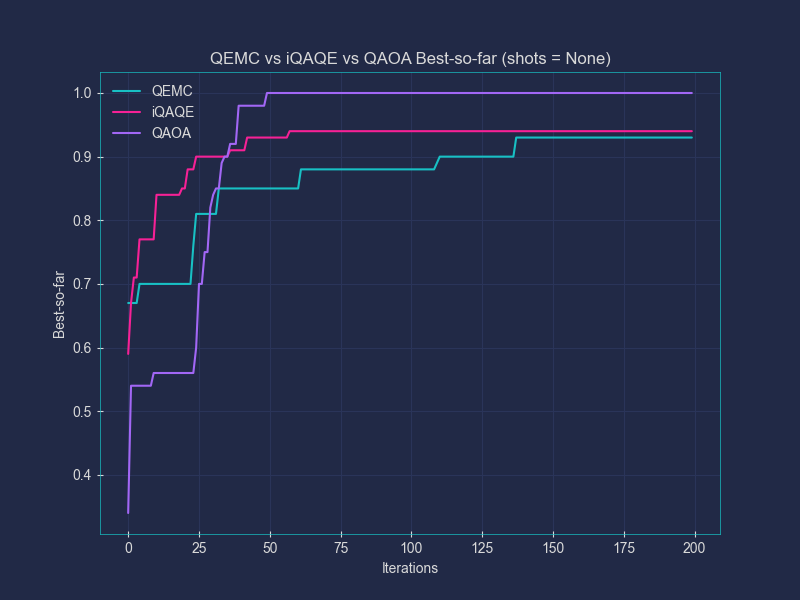
\includegraphics[width=1\textwidth]{Figures/Chapter_5/3_Comparison_shots=None.png}
      \label{fig:3_Comparison_shots=None}
  \end{subfigure}
  \hspace{-1.5em}
  \begin{subfigure}[H]{0.495\textwidth}
      \centering
      \caption*{(b) Shots = 1024}
      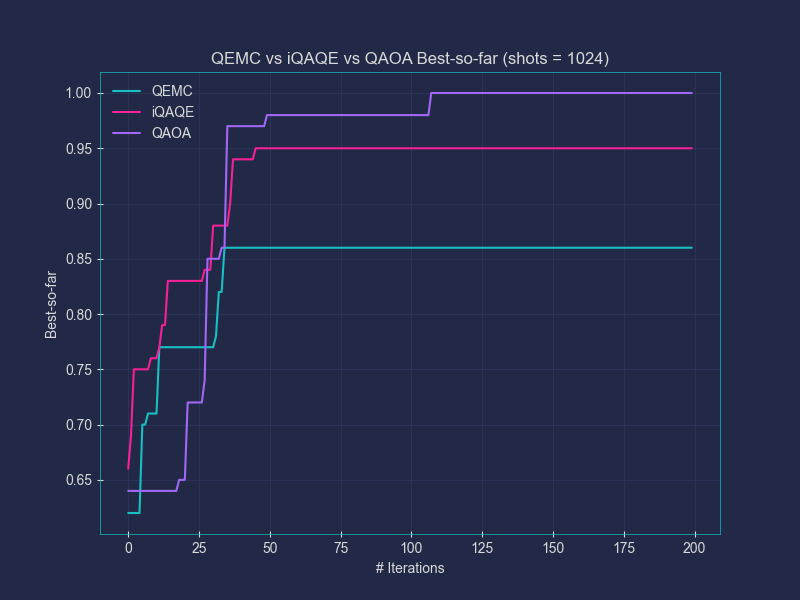
\includegraphics[width=1\textwidth]{Figures/Chapter_5/3_Comparison_shots=1024.png}
      \label{fig:3_Comparison_shots=1024}
  \end{subfigure}

  \vspace{-1.5em} % Adjust the space between the rows

  \begin{subfigure}[t]{0.495\textwidth}
      \centering
      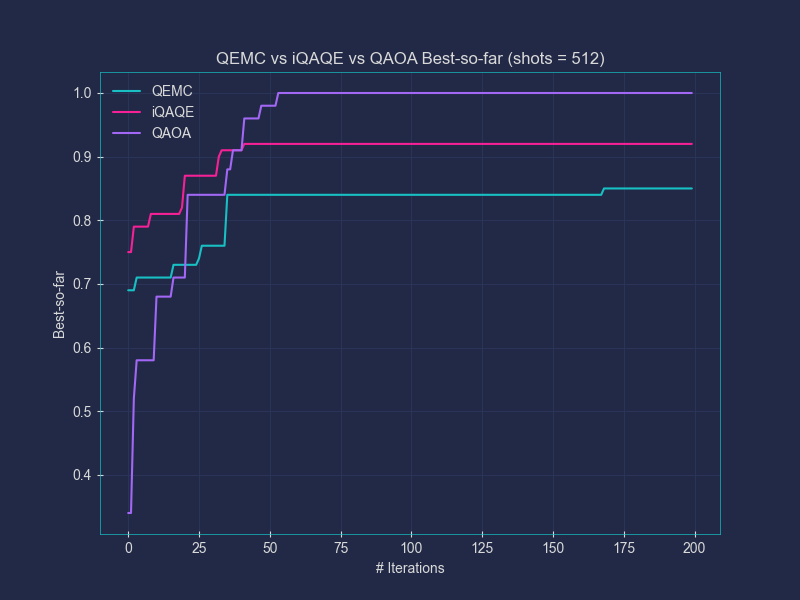
\includegraphics[width=1\textwidth]{Figures/Chapter_5/3_Comparison_shots=512.png}
      \caption*{(c) Shots = 512}
      \label{fig:3_Comparison_shots=512}
  \end{subfigure}
  \hspace{-1.5em}
  \begin{subfigure}[t]{0.495\textwidth}
      \centering
      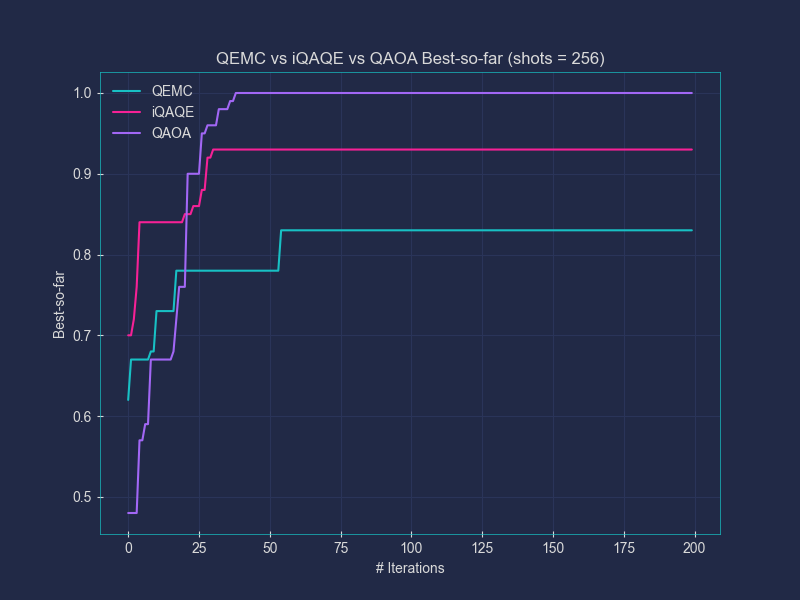
\includegraphics[width=1\textwidth]{Figures/Chapter_5/3_Comparison_shots=256.png}
      \caption*{(d) Shots = 256}
      \label{fig:3_Comparison_shots=256}
  \end{subfigure}
  
  \caption{Comparison between the $3$ \acrshort{vqa}\textcolor{gray}{s}' performances (\acrshort{qaoa}, \acrshort{qemc} and \acrshort{iqaqe}), using an infinite and finite number of shots. The best-so-far average is plotted.}
  \label{fig:3_Comparison_shots}
\end{figure}
%%%%%%%%%%%%%%%%%%%%%%%%%%%%%%%%%%%%%%%%%%%%%%%%%%%%%%%%%%%%%%%%%%%%%%%%

These plots generally align with our theoretical expectations. As \acrshort{qemc} relies heavily on a large number of shots, transitioning to a finite shot number naturally impacts the results. Surprisingly, however, \acrshort{iqaqe} seems to exhibit slightly greater resilience to this effect, despite sharing \acrshort{qemc}'s cost function and ansatz. This resilience might be attributed to the presence of multiple basis states associated with each graph node, potentially reducing the need for exhaustive sampling. If some basis states are harder to sample, the probabilities of the remaining states might adapt to compensate, as governed by the \acrshort{qemc} objective function. Nonetheless, \acrshort{qaoa} consistently outperforms both approaches, highlighting its superiority. For the same number of layers, \acrshort{qaoa}'s problem-inspired ansatz and cost function consistently yield better results. To determine if \acrshort{iqaqe} can surpass \acrshort{qaoa}'s performance, extensive testing across various combinations of parameters such as $n$, $c$, number of layers, and Adam's learning rate is necessary. This will motivate some of the grid searches we conduct later in this study. However, given the vast number of potential combinations, testing all of them is impractical. Therefore, some of the more targeted mappings/encodings explored in this work aim to constrain one or more of these variables, thereby reducing the total number of combinations for testing. Following this approach, conducting grid searches over the parameter values becomes more manageable and practical to determine the optimal settings. The subsequent sections of this chapter will detail these mapping strategies.

%%%%%%%%%%%%%%%%%%%%%%%%%%%%%%%%%%%%%%%%%%%%%%%%%%%%%%%%%%%%%%%%%%%%%%%%
\section{Polynomial Compression-type Encodings}
\label{section:Polynomial_Encodings}

At this point, driven by our earlier discussion on the nature of random-based algorithms, we begin exploring more meaningful mappings. Here, we opt to fix one or more qubits to $1$ (or $0$) while allowing the remainder to vary. The number of qubits we fix ($k$) depends on the desired order of compression. This approach not only enables the utilization of fewer qubits (if $k > 1$) but also establishes the total number of qubits to be used, simplifying subsequent grid searches over parameters. By fixing $k$ qubits, we achieve polynomial compression of order-$k$ (in the number of qubits). The total number of nodes that can be encoded in this manner is determined by $\binom{n}{k} = \frac{n!}{k!(n - k)!}$, where $n$ denotes the number of qubits. Essentially, this represents the number of ways we can select $k$ qubits from the available $n$ and set them to $1$ (or $0$), each combination encoding one graph node. Consequently, we need to ensure that $\binom{n}{k} \geq N$, where $N$ represents the number of graph nodes. This criterion guides our selection of $n$ and $k$. In practice, to determine $n$ for any $k$, we select the smallest $n$ that satisfies $\binom{n}{k} \geq N$. This yields $N = \mathcal{O}(n^k)$. Subsequently, we decide on the number of basis states to associate with each graph node, chosen from a total of $2^{n-k}$. While we could potentially utilize all $2^{n-k}$ basis states for each node (with $n-k$ free qubits), we allow for the flexibility to choose only $c \leq 2^{n-k}$. The value of $c$ requires optimization. With the mapping established, the algorithm proceeds as before, employing \acrshort{qemc}'s cost function and ansatz. Notably, we cannot use \acrshort{qaoa}'s ansatz since $n \neq N$. Due to polynomial compression, $n < N$ always, unless $k = 1$ (in which case there is no compression).






%%%%%%%%%%%%%%%%%%%%%%%%%%%%%%%%%%%%%%%%%%%%%%%%%%%%%%%%%%%%%%%%%%%%%%%%
\subsection{Basic Polynomial Compression-type iQAQE}
\label{subsection:Basic_Poly-Comp_iQAQE}


This is the simplest type of polynomial compression-based \acrshort{iqaqe} scheme. It involves fixing $k$ qubits to $1$ instead of $0$. The number of fixed qubits ($k$) is determined by the desired order of compression, as previously described. The results for $k = 2$ and $k = 3$ are shown below (Figures \ref{fig:Comparison_k2+k3_1} and \ref{fig:Comparison_k2+k3_2}). In the figures, the list cardinality is set to $4$ for both the $k = 2$ curve (\texttt{iQAQE\_k2}) and the $k = 3$ curve (\texttt{iQAQE\_k3}). Additionally, the number of layers is set to $4$ for $k = 2$ and $5$ for $k = 3$, with an Adam learning rate of $0.98$. The final curves are derived from $10$ runs of the algorithms, each with different random initial parameters. The results are compared with those of \acrshort{qaoa} and \acrshort{qemc}.

\begin{figure}[H]
  \centering
  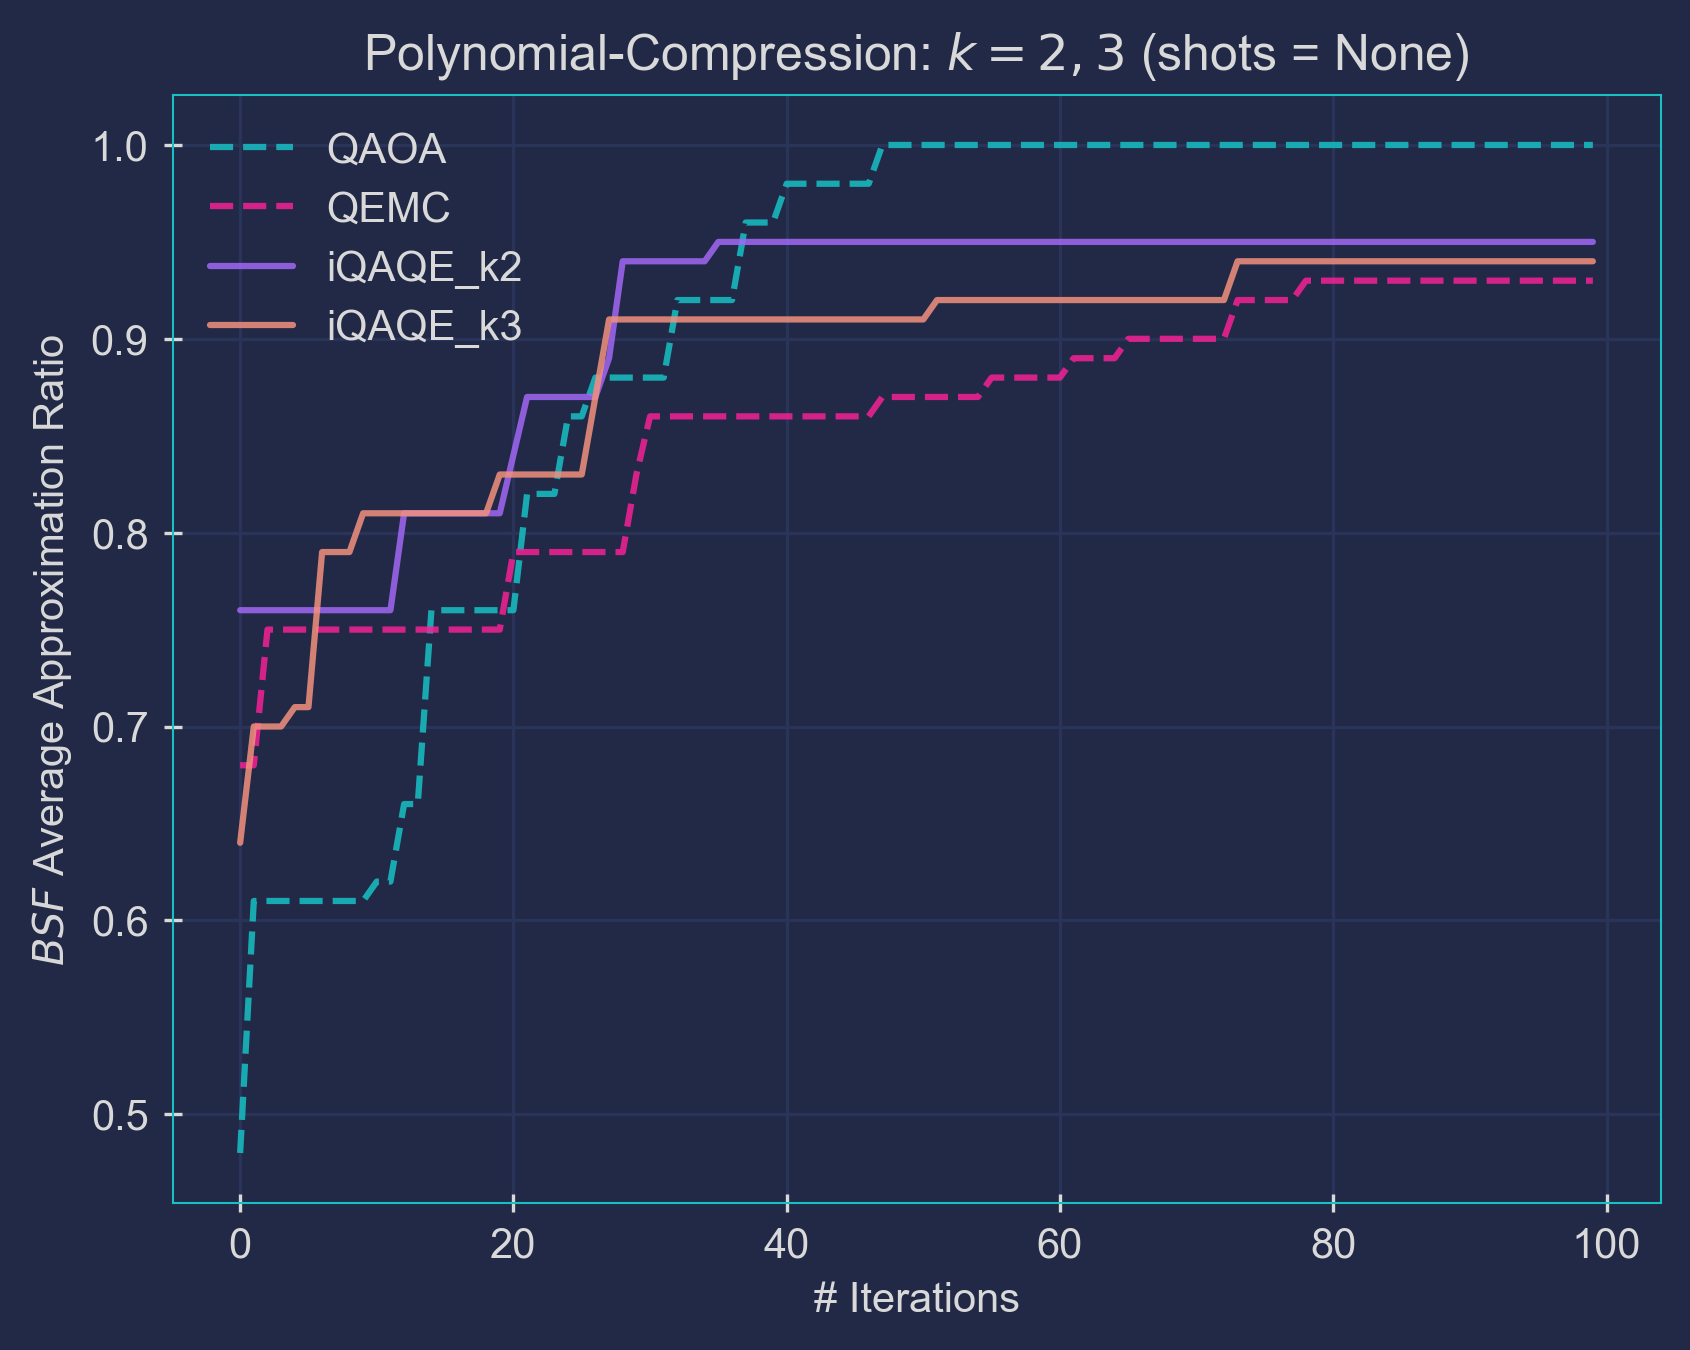
\includegraphics[width=0.70\textwidth]{Figures/Chapter_5/Polynomial_Compression_Base_k2_k3_2.png}
  \caption{\acrshort{bsf} Average Approximation Ratio \textit{vs.} iteration number for the tested \acrshort{vqa}\textcolor{gray}{s}: \acrshort{qaoa}, \acrshort{qemc}, and \acrshort{iqaqe}, using the aforementioned polynomial compression scheme. The number of layers considered were $4$ for $k = 2$ and $5$ for $k = 3$}
  \label{fig:Comparison_k2+k3_1}
\end{figure}

\begin{figure}[H]
  \centering
  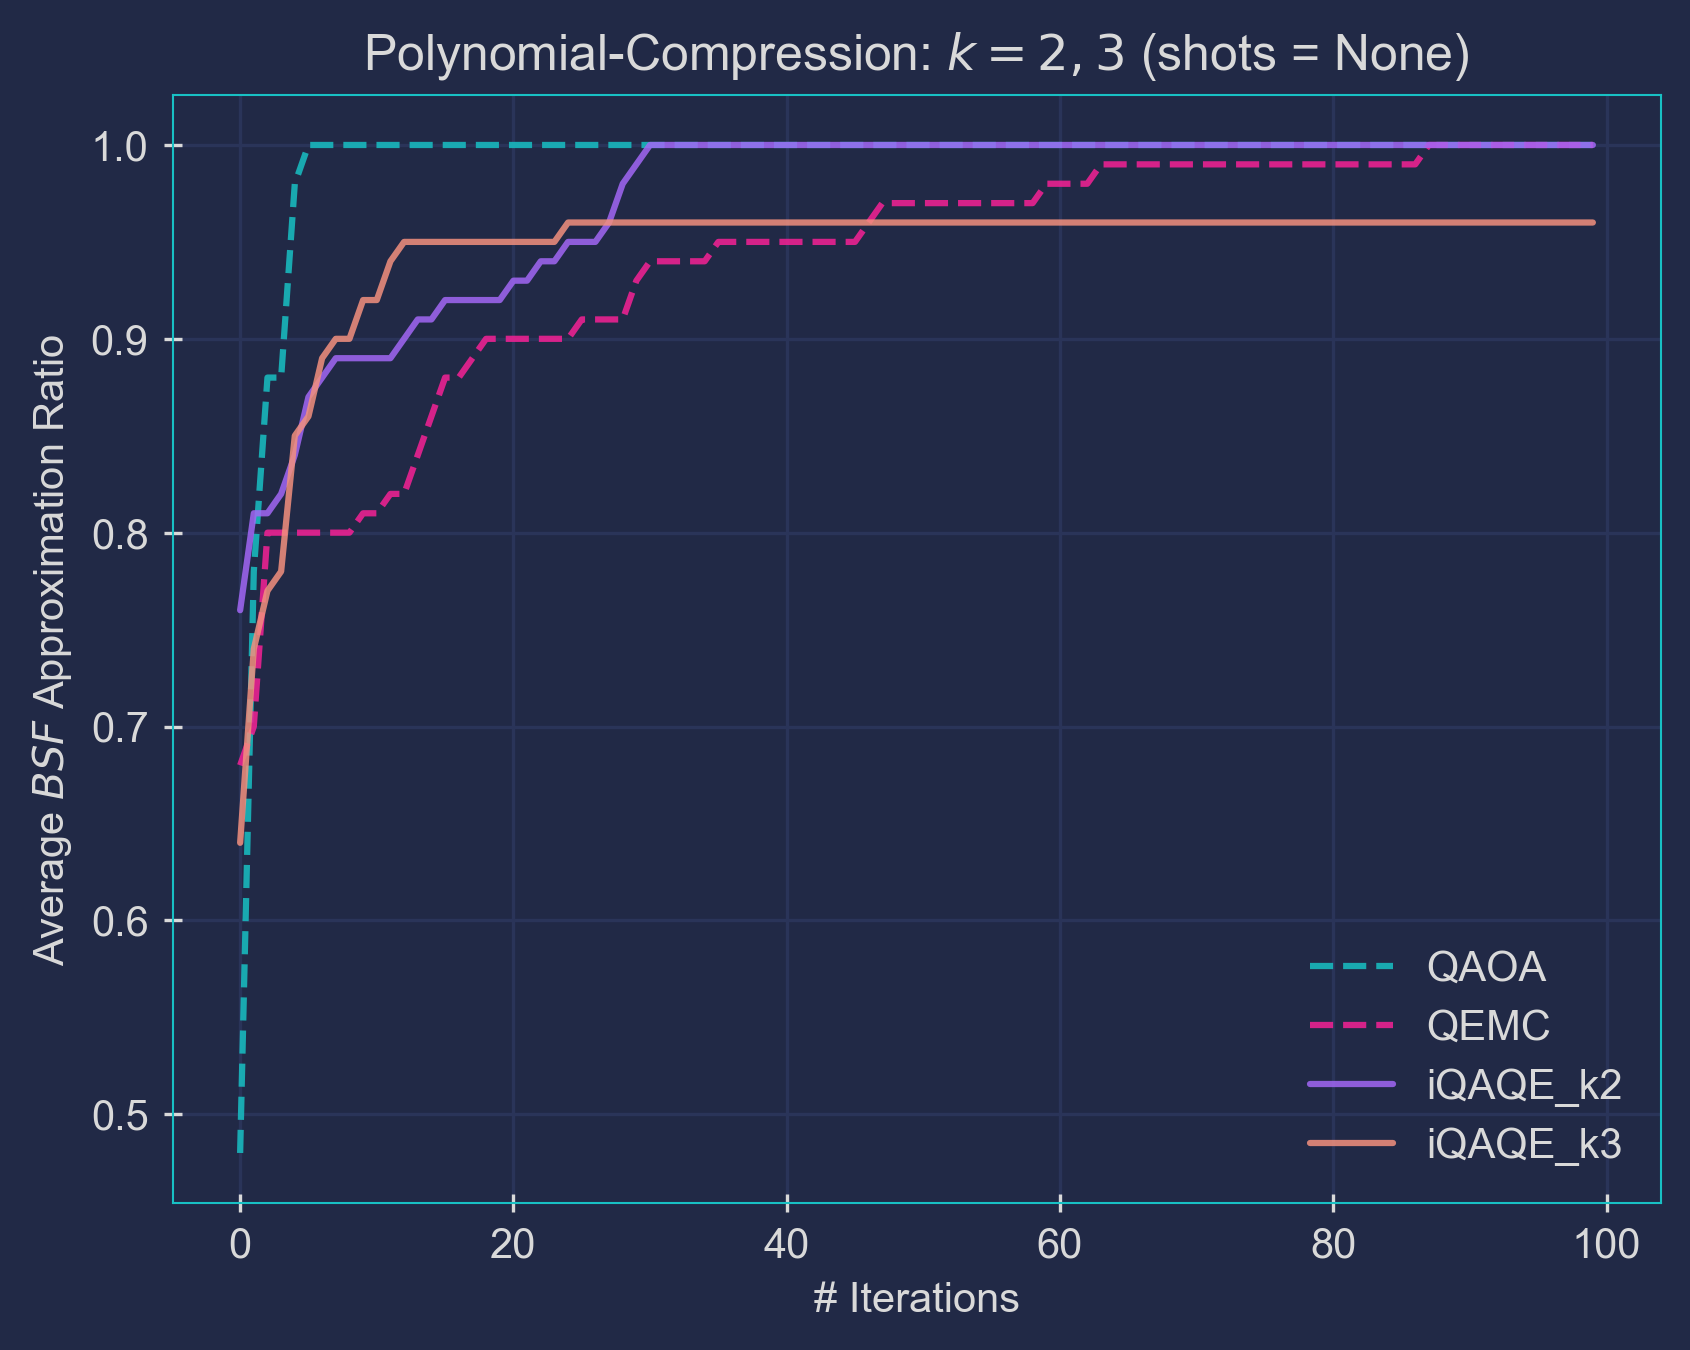
\includegraphics[width=0.70\textwidth]{Figures/Chapter_5/Polynomial_Compression_Base_k2_k3_1.png}
  \caption{Average \acrshort{bsf} Approximation Ratio \textit{vs.} iteration number for the tested \acrshort{vqa}\textcolor{gray}{s}: \acrshort{qaoa}, \acrshort{qemc}, and \acrshort{iqaqe}, using the aforementioned polynomial compression scheme. The number of layers considered were $4$ for $k = 2$ and $5$ for $k = 3$}
  \label{fig:Comparison_k2+k3_2}
\end{figure}



Notice the difference between the two figures. In the first figure, we average the curves first and then apply the \acrshort{bsf} transformation. In the second figure, we reverse the process: first applying the \acrshort{bsf} transformation to each curve and then averaging the transformed curves. The results are quite different, as illustrated. This indicates that both \acrshort{qemc} and \acrshort{iqaqe} are generally more susceptible to outliers due to particularly unlucky initial parameterizations. This is an important consideration when interpreting the forthcoming results. Often, we will choose to discard the \acrshort{bsf} average in favor of the average \acrshort{bsf}. Nonetheless, both approaches are valuable for evaluating the algorithms' properties. Additionally, in some instances, we will simply use the average. Each case will be clearly specified.

Anyways, the primary aim of this study was to assess whether different types of mappings, like the one explored here, offer advantages compared to the random case. The results in Figures \ref{fig:Comparison_k2+k3_1} and \ref{fig:Comparison_k2+k3_2} indicate that this may be the case. At the very least, they suggest that there is potential in exploring these ideas further. For example, \texttt{iQAQE\_k2} achieves a perfect approximation ratio, although it requires more iterations than \acrshort{qaoa}. Nevertheless, our method surpasses \acrshort{qemc} for $k = 2$. The results for $k = 3$ are less encouraging. However, both mappings use fewer qubits ($n = 5$) than \acrshort{qaoa} ($n = 8$), which is beneficial for implementation on practical (\acrshort{nisq}) quantum computers. The next step is to conduct grid searches over the parameters for this specific graph instance to determine if we can consistently achieve better performance than \acrshort{qaoa}. This might provide further insights into the underlying principles of the algorithm's performance.

% k=2:
\begin{figure*}[ht!]
  \centering
  \begin{subfigure}[b]{0.325\textwidth}
      \centering
      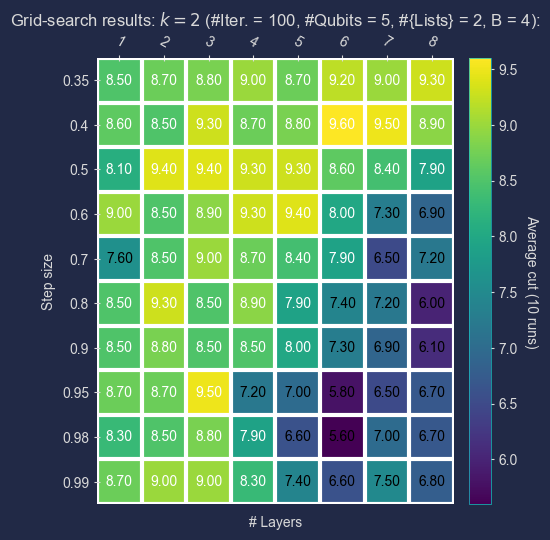
\includegraphics[width=1\textwidth]{Figures/Chapter_5/k=2(Grid_Search)/iQAQE_k2_Grid_Search_step_size_n_layers_c=2.png}
      \caption{\texttt{k = 2; c = 2}}
      \label{fig:k=2;c=2}
  \end{subfigure}
  \hfill
  \begin{subfigure}[b]{0.325\textwidth}
      \centering
      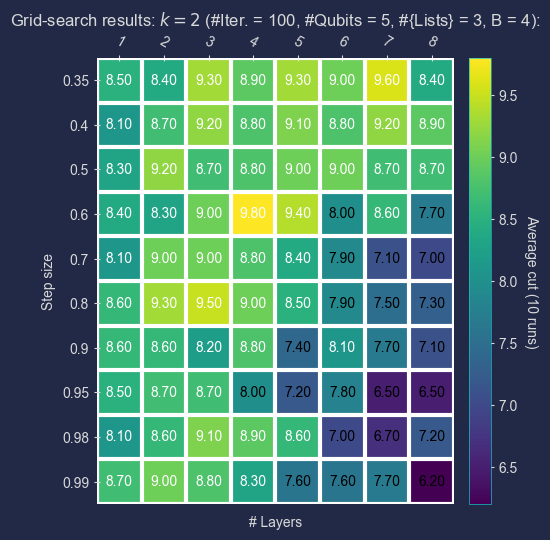
\includegraphics[width=1\textwidth]{Figures/Chapter_5/k=2(Grid_Search)/iQAQE_k2_Grid_Search_step_size_n_layers_c=3.png}
      \caption{\texttt{k = 2; c = 3}}
      \label{fig:k=2;c=3}
  \end{subfigure}
  \hfill
      \begin{subfigure}[b]{0.325\textwidth}
      \centering
      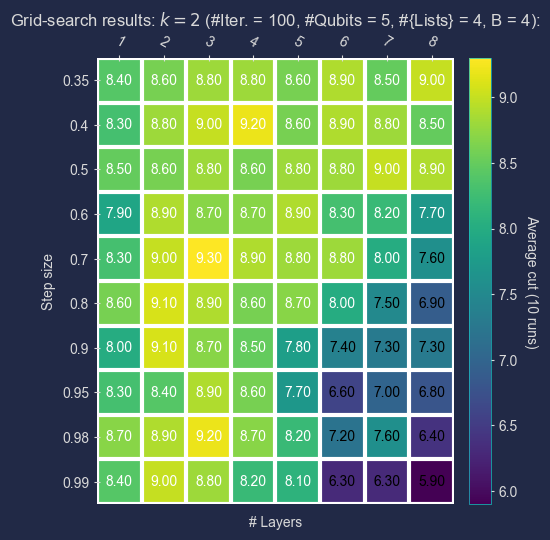
\includegraphics[width=1\textwidth]{Figures/Chapter_5/k=2(Grid_Search)/iQAQE_k2_Grid_Search_step_size_n_layers_c=4.png}
      \caption{\texttt{k = 2; c = 4}}
      \label{fig:k=2;c=4}
  \end{subfigure}
  \bigskip
  \begin{subfigure}[b]{0.325\textwidth}
      \addtocounter{subfigure}{3} % Added <<
      \centering
      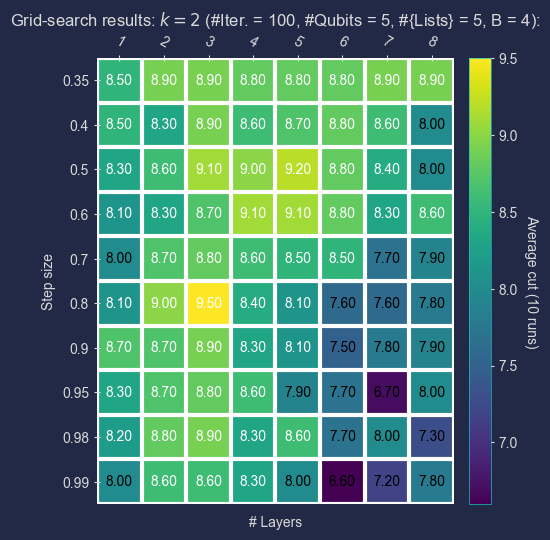
\includegraphics[width=1\textwidth]{Figures/Chapter_5/k=2(Grid_Search)/iQAQE_k2_Grid_Search_step_size_n_layers_c=5.png}
      \caption{\texttt{k = 2; c = 5}}
      \label{fig:k=2;c=5}
  \end{subfigure}
  \hfill
  \begin{subfigure}[b]{0.325\textwidth}
      \centering
      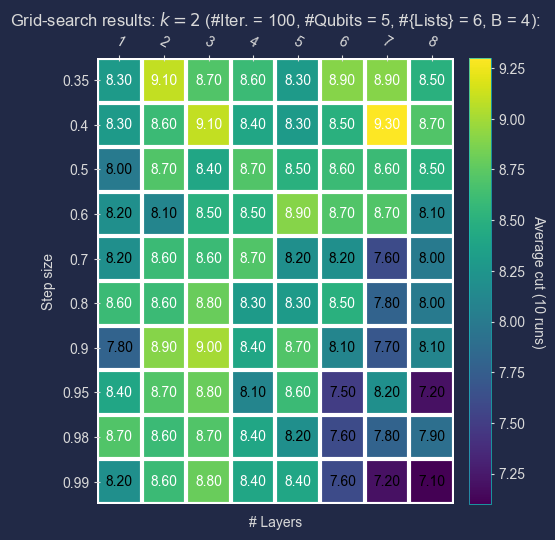
\includegraphics[width=1\textwidth]{Figures/Chapter_5/k=2(Grid_Search)/iQAQE_k2_Grid_Search_step_size_n_layers_c=6.png}
      \caption{\texttt{k = 2; c = 6}}
      \label{fig:k=2;c=6}
  \end{subfigure}
  \hfill
  \begin{subfigure}[b]{0.325\textwidth}
      \centering
      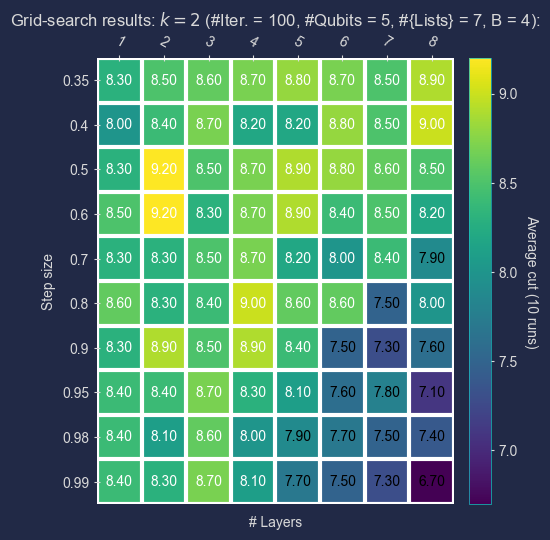
\includegraphics[width=1\textwidth]{Figures/Chapter_5/k=2(Grid_Search)/iQAQE_k2_Grid_Search_step_size_n_layers_c=7.png}
      \caption{\texttt{k = 2; c = 7}}
      \label{fig:k=2;c=7}
  \end{subfigure}
  \caption{Basic Polynomial Compression-type \acrshort{iqaqe} – Grid search, using $k=2$. All the simulations were done using an infinite number of shots (\texttt{shots = None}), and each value consists of the average of $10$ \acrshort{iqaqe} instances, using different random initial parameters.}
  \label{fig:k=2}
\end{figure*}

% k=3:
\begin{figure*}[ht!]
  \centering
  \begin{subfigure}[b]{0.475\textwidth}
      \centering
      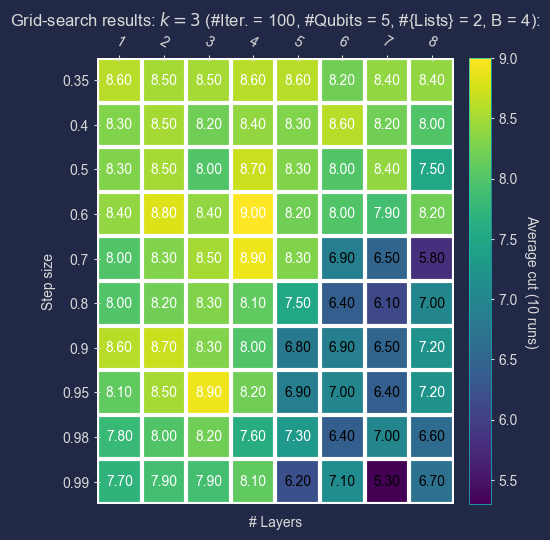
\includegraphics[width=1\textwidth]{Figures/Chapter_5/k=3(Grid_search)/iQAQE_k3_Grid_Search_step_size_n_layers_c=2.png}
      \caption{\texttt{k = 3; c = 2}}
      \label{fig:k=3;c=2}
  \end{subfigure}
  \hfill
  \begin{subfigure}[b]{0.475\textwidth}
      \centering
      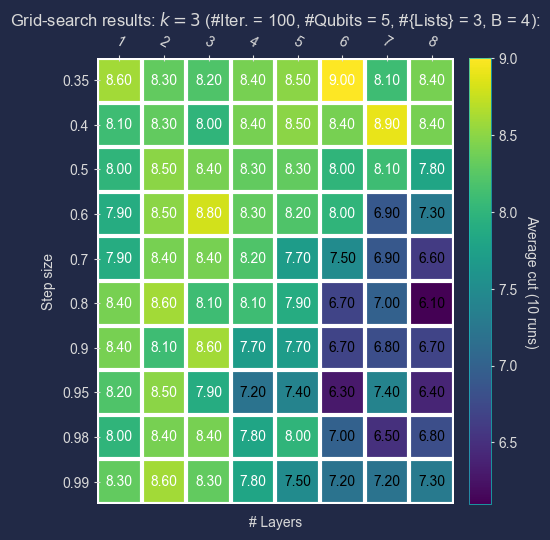
\includegraphics[width=1\textwidth]{Figures/Chapter_5/k=3(Grid_search)/iQAQE_k3_Grid_Search_step_size_n_layers_c=3.png}
      \caption{\texttt{k = 3; c = 3}}
      \label{fig:k=3;c=3}
  \end{subfigure}
  \caption{Basic Polynomial Compression-type \acrshort{iqaqe} – Grid search, using $k=3$. All the simulations were done using an infinite number of shots (\texttt{shots = None}), and each value consists of the average of $10$ \acrshort{iqaqe} instances, using different random initial parameters.}
  \label{fig:k=3}
\end{figure*}

The results of the grid searches conducted for $k=2$ and $k=3$ are present in Figures \ref{fig:k=2} and \ref{fig:k=3}. Various values were explored for the parameters: \texttt{step\_size\_list = [0.35, 0.4, 0.5, 0.6, 0.7, 0.8, 0.9, 0.95, 0.98, 0.99]}, \texttt{n\_layers} ranging from $1$ to $8$, and \texttt{c} varying from $2$ to $(2^{\texttt{n - k}} - 1)$, for $k=2, 3$, where \texttt{n\_layers} and \texttt{c} are integers. Notably, all simulations for the grid searches were executed with an infinite number of shots (\texttt{shots = None}). Additionally, this time, we utilized the average curve (from $10$ instances) instead of the average best-so-far curve. This choice was made to evaluate the overall performance of the algorithm rather than focusing solely on the best-performing instances. Each run continued until convergence (\texttt{abs\_tol <= 1e-5}) or \texttt{max\_iter = 1000} was reached, followed by recording the final partition's cut. The objective was to identify any discernible patterns in the grid search to enhance the scheme's performance. However, no apparent pattern emerged, highlighting a recurring challenge in this work: the abundance of hyperparameters makes it challenging to optimize results through straightforward means. Later, we will explore employing a more intricate machine learning scheme to address this challenge. For now, we proceed with a different approach.

% Then, it's grid-search(es).
% After that, recovery of the QAOA limit.
% Finally, other values of $k$. Actually, what I have now should be under this subsubsection, instead of the one above. I'll fix this, tomorrow.

% Then, I can quickly go through correlation-based iQAQE and fixed-parity iQAQE. I'll leave this for tomorrow, as well.

% Afterwards, Extended-QEMC, and all the other surrounding topics.





%%%%%%%%%%%%%%%%%%%%%%%%%%%%%%%%%%%%%%%%%%%%%%%%%%%%%%%%%%%%%%%%%%%%%%%%
\subsubsection*{Recovering the QAOA limit ($k = 1$)}
\label{subsubsection:QAOA-Limit_iQAQE}


Next, we tested whether we could recover the \acrshort{qaoa} limit using \acrshort{iqaqe}'s algorithm with what we call the \acrshort{qaoa} mapping for this scheme. This mapping involves using the same number of qubits as there are nodes (as in standard \acrshort{qaoa}) and assigning $2^{n-1}$ basis states to each graph node. For each graph node, a different qubit is fixed to $1$, while the remaining $n - 1$ qubits are free to vary, resulting in $2^{n-1}$ basis states per node. The rest of the algorithm remains unchanged, employing \acrshort{qemc}'s ansatz and cost function. The nodes' probabilities are derived from the normalized sum of the probabilities of their associated basis states. This approach was motivated by our desire to better understand \acrshort{iqaqe}'s properties and behavior. Previously, we observed (Figure \ref{fig:3_Comparison_shots}) that \acrshort{iqaqe}'s performance seemed to fall between that of \acrshort{qaoa} and \acrshort{qemc}, which is intuitive, as it is designed as an interpolation between the two. To further test this behavior, we used \acrshort{qaoa}'s mapping to see how closely we could approach \acrshort{qaoa}'s performance levels, which have been the best so far. The following results were obtained, focusing only on analytical simulations (i.e., infinite shots) – We employ the average curve obtained from $10$ runs, as we did in the previous grid search:

\begin{figure}[H]
  \centering
  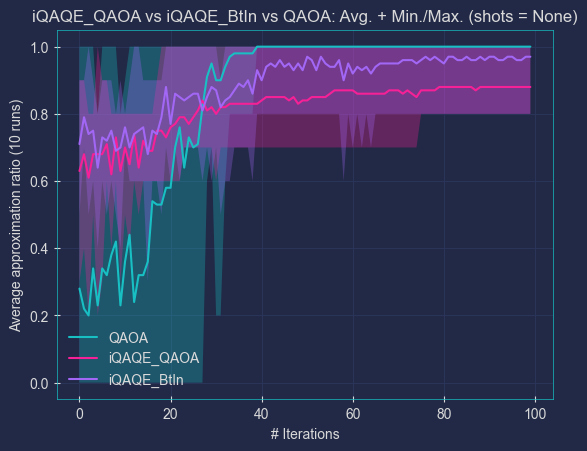
\includegraphics[width=0.70\textwidth]{Figures/Chapter_5/iQAQE_QAOA.png}
  \caption{Average approximation ratio ($\pm \sigma$) $vs$ iteration number, for the three tested \acrshort{vqa}\textcolor{gray}{s}: \texttt{QAOA}, \texttt{iQAQE\_QAOA} (as described above) and \texttt{iQAQE\_BtIn}. The latter stands for \acrshort{iqaqe}, with better initialization. This corresponds to the same mapping as the one in Figure \ref{fig:3_Comparison_shots}.}
  \label{fig:iQAQE_QAOA}
\end{figure}

This realization led us to understand that we cannot expect to replicate \acrshort{qaoa}'s outstanding performance on this graph simply by using a \acrshort{qaoa}-type encoding. After all, we are still relying on \acrshort{qemc}'s cost function and ansatz, so this outcome is not entirely surprising. Moreover, to add to the challenge, we found that \texttt{iQAQE\_QAOA}'s performance can even be surpassed by another random, non-specific mapping, highlighting how far we are from achieving \acrshort{qaoa}-like results.

In an effort to bridge this gap, we attempted to integrate \acrshort{qaoa}'s ansatz into the scheme, alongside the \acrshort{qaoa}-type encoding. However, after extensive testing, we realized this approach is not feasible. Here's why: using both elements together with the node probability encoding (as a normalized sum of their associated basis states' probabilities) causes the \acrshort{qemc} cost function to become independent of the ansatz's parameters\footnote{To verify this, we performed analytical calculations for a simple toy model: a graph with two nodes connected by a single edge. The results generalize to larger graphs.}. This means we cannot proceed with training, rendering the scheme ineffective. Thus, implementing this approach in its current form is not possible. For it to be successful, other aspects would need to change, such as the cost function or the method of deriving node probabilities from basis states' probabilities, which is the main issue here.









%%%%%%%%%%%%%%%%%%%%%%%%%%%%%%%%%%%%%%%%%%%%%%%%%%%%%%%%%%%%%%%%%%%%%%%%
% \subsection{Parity-like QAOA}
% \label{subsection:Parity_QAOA}

% Parity-like QAOA schemes and their results.

% % Send this to Chapter 6, instead.





%%%%%%%%%%%%%%%%%%%%%%%%%%%%%%%%%%%%%%%%%%%%%%%%%%%%%%%%%%%%%%%%%%%%%%%%
\subsection{Correlation-based iQAQE}
\label{subsection:Correlation_iQAQE}

This scheme closely resembles what was previously discussed in subsection \ref{subsection:Basic_Poly-Comp_iQAQE}. The key distinction lies in the inclusion of the possibility for both $0$'s and $1$'s to be fixed. Consequently, the scheme aims to identify correlations among the different qubits, wherein "correlations" denote identical colors. In other words, the constructed lists regard the $k$ fixed qubits as positively correlated, meaning they are either all set to $1$ or all set to $0$. This approach was inspired by the notion that by identifying correlations between nodes, it becomes feasible to color the entire graph as long as one node is initially colored. Although seeking correlations between qubits, as done here, differs from seeking correlations between nodes, we anticipated that it might yield promising results to some extent. In this scenario, the color of each node is determined by the probability that its $k$ associated qubits are all positively correlated.

To delve deeper into the properties and characteristics of this scheme, we conducted a thorough formal analysis, exploring its limits by considering scenarios where $k$ ranges from $1$ to $n$ qubits, covering the entire spectrum. Our primary objective was to ascertain if we could formulate this correlation-based \acrshort{iqaqe} scheme in a manner that truly interpolates between \acrshort{qaoa} and \acrshort{qemc}. We aimed to determine if we could retrieve both algorithms by adjusting the parameters accordingly. However, with this correlation-based scheme, we not only cannot recover \acrshort{qaoa}, but we also fail to retrieve \acrshort{qemc}. Thus, this does not represent an interpolation between the two algorithms.

Likewise, earlier, we loosely referred to the \acrshort{iqaqe} Framework as an interpolation. However, upon closer scrutiny, this characterization seems inaccurate. While it is possible to recover the \acrshort{qemc} limit\footnote{Simply utilize the appropriate number of qubits and select one unique basis state for each node.}, the same cannot be said for \acrshort{qaoa}, as we have observed before.

Additionally, we provide the results of numerical simulations applied to the standard $8$-node graph.

\begin{figure}[H]
  \centering
  \begin{subfigure}[t]{0.495\textwidth}
      \centering
      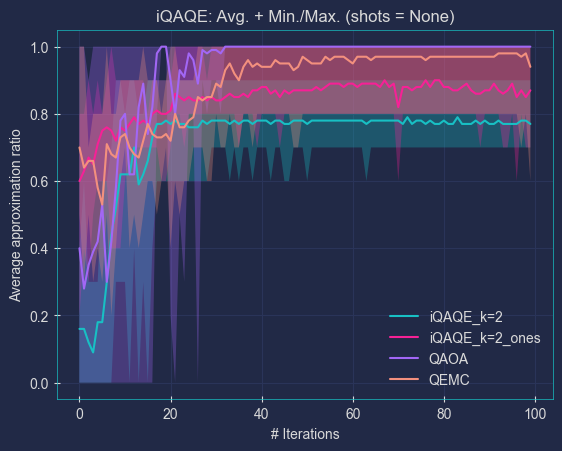
\includegraphics[width=1\textwidth]{Figures/Chapter_5/Correlation-based/k=2(Reg.+Ones).png}
      \caption{\raggedright Comparison of Correlation-based \acrshort{iqaqe} for $k=2$ with results from \acrshort{qaoa}, \acrshort{qemc}, and the previous Basic Polynomial Compression-type iQAQE\footnotemark{} (\texttt{iQAQE\_k=2\_ones}).}
      \label{fig:Correlation/k=2}
  \end{subfigure}
  \hfill
  \begin{subfigure}[t]{0.495\textwidth}
      \centering
      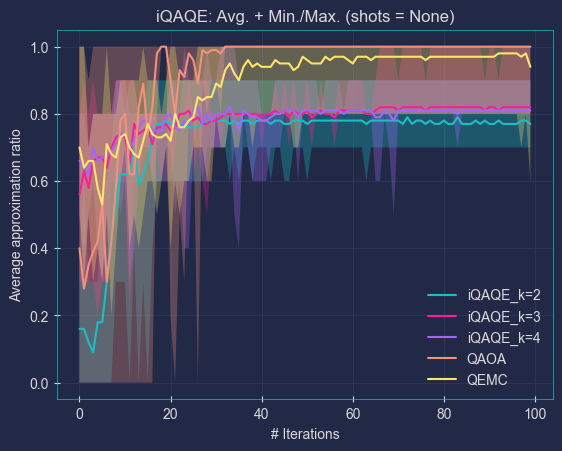
\includegraphics[width=1\textwidth]{Figures/Chapter_5/Correlation-based/k=2_3_4.png}
      \caption{Comparison of Correlation-based \acrshort{iqaqe} results for $k=2, 3$, and $4$ with outcomes from \acrshort{qaoa} and \acrshort{qemc}.}
      \label{fig:Correlation/k=2,3,4}
  \end{subfigure}
  \caption{Correlation-based polynomial-type compression scheme ($k=2, 3$ and $4$): numerical simulations for the usual $8$-node graph.}
  \label{fig:Correlation-based}
\end{figure}

\footnotetext[\value{footnote}]{This refers to the scenario where only $1$'s are fixed, not $0$'s.}

\clearpage

\begin{figure}[H]
  \centering
  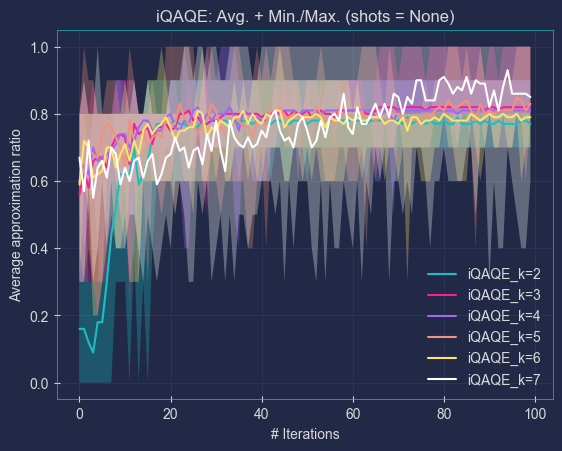
\includegraphics[width=\textwidth]{Figures/Chapter_5/Correlation-based/All_k's.png}
  \caption{Correlation-based polynomial-type compression scheme ($k = 2, 3, 4, 5, 6$ and $7$): numerical simulations for the usual $8$-node graph.}
  \label{fig:All_k's}
\end{figure}

Note that we once again use the average approximation ratio from $10$ runs, each with different random initial parameters. Additionally, we plot the average, with the shaded region representing the maximum and minimum obtained approximation ratios. Performance-wise, this scheme does not fare well. It is significantly outperformed by \acrshort{qaoa}, \acrshort{qemc}, and the basic polynomial compression-type \acrshort{iqaqe}. We also compared the results for all possible values of $k$ (Figure \ref{fig:All_k's}). It turns out that the specific value of $k$ is not very meaningful, as performance is quite similar across all values.

The underperformance is likely due to our doubling the number of basis states in each sublist. This encoding results in each pair of sublists having a $50\%$ overlap, similar to the Basic Polynomial Compression-type \acrshort{iqaqe}. However, with twice\footnote{Either $0$'s or $1$'s can be fixed.} the number of basis states this time, the number of overlapping basis states is significantly higher. This increase means that more states are shared by multiple nodes. When the overlap is too large, it becomes more challenging to adjust the color of one node without affecting the others. We believe this to be the main reason for the underperformance. We will be mindful of this in the design of future schemes.

% One of these schemes allowed to easily recover QEMC in one of its limits. Try to figure out what that was.

% Analytical analysis: do I even want to include this here? It didn't really amount to much, in the end... I'll have to think about this.





%%%%%%%%%%%%%%%%%%%%%%%%%%%%%%%%%%%%%%%%%%%%%%%%%%%%%%%%%%%%%%%%%%%%%%%%
\subsection{Fixed-Parity iQAQE}
\label{subsection:Fixed-Parity_iQAQE}

% Mention that this is a 'heuristic'. It's not a strict rule, but it's a good guideline.

In this section, we present another heuristic method for mapping the basis states to the nodes. Although it is similar to the previous one, this time we \textbf{fixed the parity of the selected $k$ qubits to be even}. Parity is determined by the number of 1's: if the count is even, the parity is even; otherwise, it is odd. For instance, for $k=3$ (with \texttt{n\_qubits = 5}), the lists would take the form: (Keep in mind that we are using an $8$-node graph.)

% Remeber that 'k=2' is the same as the previous correlation-based! Mention this in the text!

\begin{multicols}{2}
  \begin{enumerate}
    \item $\left\{\ket{000\text{xx}}, \ket{011\text{xx}}, \ket{101\text{xx}}, \ket{110\text{xx}}\right\}$;
    \item $\left\{\ket{00\text{xx}0}, \ket{01\text{xx}1}, \ket{10\text{xx}1}, \ket{11\text{xx}0}\right\}$;
    \item $\left\{\ket{0\text{xx}00}, \ket{0\text{xx}11}, \ket{1\text{xx}01}, \ket{1\text{xx}10}\right\}$;
    \item $\left\{\ket{\text{xx}000}, \ket{\text{xx}011}, \ket{\text{xx}101}, \ket{\text{xx}110}\right\}$;
    \item $\left\{\ket{\text{x}0\text{x}00}, \ket{\text{x}0\text{x}11}, \ket{\text{x}1\text{x}01}, \ket{\text{x}1\text{x}10}\right\}$;
    \item $\left\{\ket{\text{x}00\text{x}0}, \ket{\text{x}01\text{x}1}, \ket{\text{x}10\text{x}1}, \ket{\text{x}11\text{x}0}\right\}$;
    \item $\left\{\ket{\text{x}000\text{x}}, \ket{\text{x}011\text{x}}, \ket{\text{x}101\text{x}}, \ket{\text{x}110\text{x}}\right\}$;
    \item $\left\{\ket{0\text{x}0\text{x}0}, \ket{0\text{x}1\text{x}1}, \ket{1\text{x}0\text{x}1}, \ket{1\text{x}1\text{x}0}\right\}$.
  \end{enumerate}
\end{multicols}
\noindent Once again, numerical simulations were performed, and the obtained results are presented below (Figure \ref{fig:Fixed-parity}). Although the performance is still not quite on par with \acrshort{qaoa}, it is significantly better than in the previously considered scenario. Note that the case where $k=2$ corresponds to the previous correlation-based scheme. For $k=2$, requiring the pair to be even is equivalent to requiring them to be the same (either both $0$ or both $1$), which explains the similarity in results. This similarity is apparent in the less favorable outcomes shown for $k=2$ in Figure \ref{fig:Fixed-parity}, which qualitatively match those in Figures \ref{fig:Correlation-based} and \ref{fig:All_k's}. However, when we allow for $k>2$, the performance improves significantly, likely due to the reduced overlap between the basis states associated with different nodes.

A keen observer might notice that this scheme's results also allow for generating the MaxCut partition, as shown by the shaded pink region in Figure \ref{fig:Fixed-parity/k=2,3,4} for $k=3$. These shaded regions depict the maximum and minimum cuts achieved out of the $10$ runs. This reveals that, despite the greater variability and lower average performance than \acrshort{qaoa}, the algorithm can achieve the MaxCut partition in some runs. In practice, this is crucial. When running the algorithm $10$ times, our main interest is in the best outcome. This highlights the potential of this heuristic scheme.

\begin{figure}[hb!]
  \centering
  \begin{subfigure}[t]{0.495\textwidth}
      \centering
      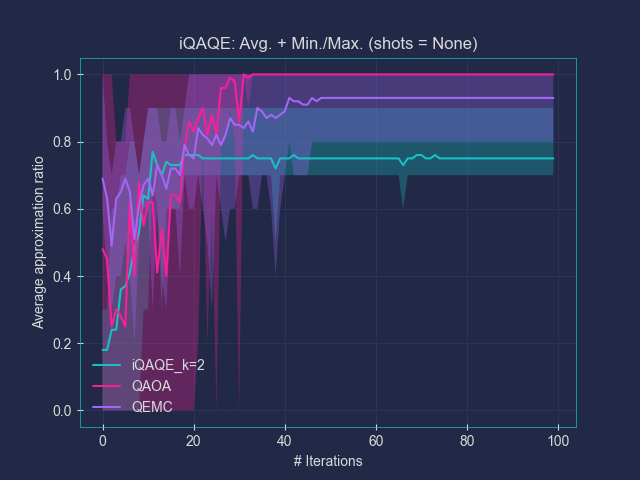
\includegraphics[width=1\textwidth]{Figures/Chapter_5/Fixed-parity/k=2(8-node).png}
      \caption{Fixed-parity \acrshort{iqaqe} for $k=2$ compared with the results from \acrshort{qaoa} and \acrshort{qemc} ($8$-node graph).}
      \label{fig:Fixed-parity/k=2}
  \end{subfigure}
  \hfill
  \begin{subfigure}[t]{0.495\textwidth}
      \centering
      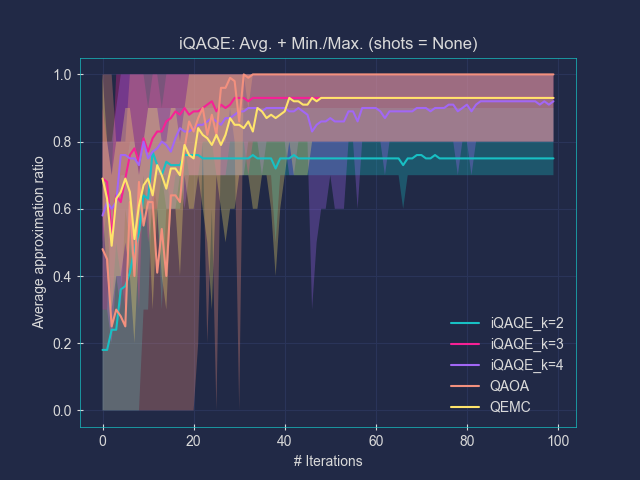
\includegraphics[width=1\textwidth]{Figures/Chapter_5/Fixed-parity/k=2_3_4(8-node).png}
      \caption{Fixed-parity \acrshort{iqaqe} for $k=2, 3$, and $4$ compared with the results from \acrshort{qaoa} and \acrshort{qemc} ($8$-node graph).}
      \label{fig:Fixed-parity/k=2,3,4}
  \end{subfigure}
\end{figure}

\clearpage

\begin{figure}[ht!]
  \addtocounter{figure}{-1} % Added <<
  \centering
  \begin{subfigure}[b]{1\textwidth}
      \addtocounter{subfigure}{2} % Added <<
      \centering
      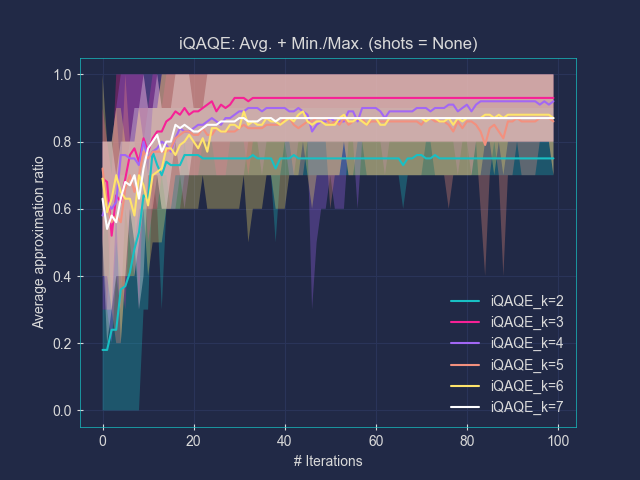
\includegraphics[width=1\textwidth]{Figures/Chapter_5/Fixed-parity/All_k's(8-node).png}
      \caption{Fixed-parity \acrshort{iqaqe} for all values of $k = 2, 3, 4, 5, 6$, and $7$ ($8$-node graph).}
      \label{fig:Fixed-parity/All_k's}
  \end{subfigure}
  \caption{Fixed-parity polynomial-type compression scheme: numerical simulations for the usual $8$-node graph.}
  \label{fig:Fixed-parity}
\end{figure}

Furthermore, numerical simulations were carried out on a random $16$-node graph\footnote{This graph was generated using NetworkX's \texttt{nx.gnm\_random\_graph(n, m)} with \texttt{n = 16} nodes and \texttt{m = 32} edges, using \texttt{np.random.seed} set to \texttt{44}.}. Considering the satisfactory performance observed with the previous $8$-node graph, we were intrigued to assess the algorithm's performance on a larger scale. The results are now presented (Figure \ref{fig:Fixed-parity(16_node)}).

\begin{figure*}[ht!]
  \centering
  \begin{subfigure}[t]{0.495\textwidth}
      \centering
      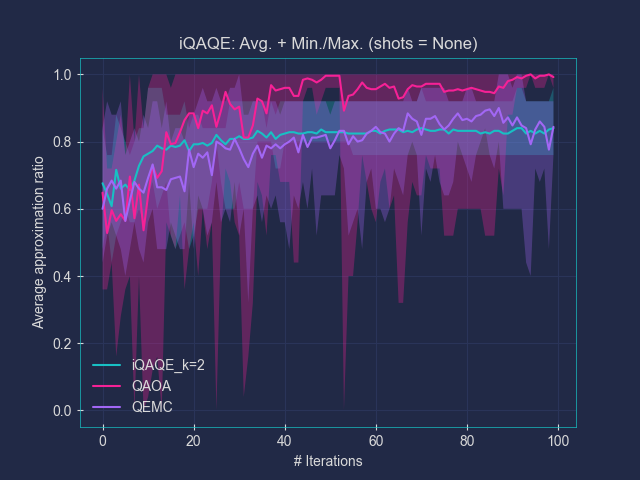
\includegraphics[width=1\textwidth]{Figures/Chapter_5/Fixed-parity/k=2(16-node).png}
      \caption{Fixed-parity \acrshort{iqaqe} for $k=2$ compared with the results from \acrshort{qaoa} and \acrshort{qemc} ($16$-node graph).}
      \label{fig:Fixed-parity/k=2(16_node)}
  \end{subfigure}
  \hfill
  \begin{subfigure}[t]{0.495\textwidth}
      \centering
      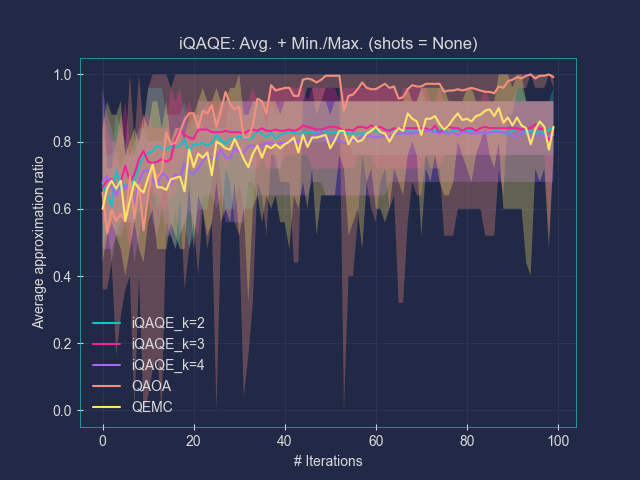
\includegraphics[width=1\textwidth]{Figures/Chapter_5/Fixed-parity/k=2_3_4(16-node).png}
      \caption{Fixed-parity \acrshort{iqaqe} for $k=2, 3$, and $4$ compared with the results from \acrshort{qaoa} and \acrshort{qemc} ($16$-node graph).}
      \label{fig:Fixed-parity/k=2,3,4(16_node)}
  \end{subfigure}
\end{figure*}

\clearpage

\begin{figure*}[ht!]
  \addtocounter{figure}{-1} % Added <<
  \centering
  \begin{subfigure}[b]{\textwidth}
      \addtocounter{subfigure}{2} % Added <<
      \centering
      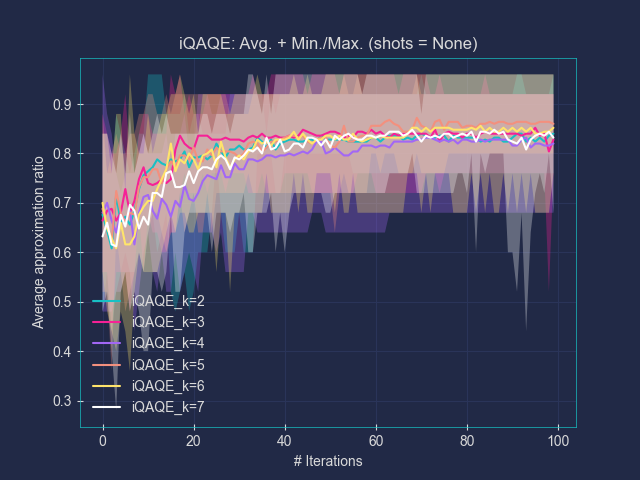
\includegraphics[width=1\textwidth]{Figures/Chapter_5/Fixed-parity/All_k's(16-node).png}
      \caption{Fixed-parity \acrshort{iqaqe} for all values of $k = 2, 3, 4, 5, 6$, and $7$ ($16$-node graph).}
      \label{fig:All_k's(16_node)}
  \end{subfigure}
  \caption{Fixed-parity polynomial-type compression scheme: numerical simulations for a $16$-node graph.}
  \label{fig:Fixed-parity(16_node)}
\end{figure*}

The previously identified trends are also apparent here. However, the performance now seems insufficient to achieve the MaxCut partition (determined by brute-force), as illustrated by the shaded areas in Figure \ref{fig:All_k's(16_node)}: the average \acrshort{ar} never quite reaches $1$. Moreover, for this graph, varying the value of $k$ does not significantly impact performance. Hence, it is advisable to choose the value of $k$ that requires the fewest qubits. In this instance, $k=3$ is optimal, needing only \texttt{n\_qubits = 6}, since $\binom{6}{3} = 20 \geq 16$.

%%%%%%%%%%%%%%%%%%%%%%%%%%%%%%%%%%%%%%%%%%%%%%%%%%%%%%%%%%%%%%%%%%%%%%%%
% \section{Other Exploratory Ideas}
% \label{section:Exploratory_Ideas}

% Other exploratory ideas and their results.

% % Send this to Chapter 6, instead.




%%%%%%%%%%%%%%%%%%%%%%%%%%%%%%%%%%%%%%%%%%%%%%%%%%%%%%%%%%%%%%%%%%%%%%%%
% \subsection{Tranche-based Oracle colouring}
% \label{section:Oracle_colouring}

% Tranche-based Oracle colouring schemes and their results.

% % Send this to Chapter 6, instead.




%%%%%%%%%%%%%%%%%%%%%%%%%%%%%%%%%%%%%%%%%%%%%%%%%%%%%%%%%%%%%%%%%%%%%%%%
\section{Extended-QEMC}
\label{section:Extended_QEMC}

% Extended-QEMC scheme and variations thereof, and their results.

Amid the various schemes we've attempted, I've devised an extension to the standard \acrshort{qemc} scheme. This new approach enhances \acrshort{qemc} by incorporating $m$ additional qubits beyond the usual $\lceil\log_2(n)\rceil$ qubits required for $n$ graph nodes.

%%%%%%%%%%%%%%%%%%%%%%%%%%%%%%%%%%%%%%%%%%%%%%%%%%%%%%%%%%%%%%%%%%%%%%%%
\subsection{Unmodified Extended-QEMC}
\label{subsection:Vanilla_Extended_QEMC}

Rather than associating a single basis state with each graph node, it assigns $2^m$ basis states per node. Importantly, similar to \acrshort{qemc}, the sets of basis states associated with different nodes do not overlap. This non-overlapping property is crucial, as we suspect that significant overlap between nodes' lists might contribute to the subpar performance observed in the correlation-based and fixed-parity \acrshort{iqaqe}\textcolor{gray}{s}.

This extended scheme can be implemented within the \acrshort{iqaqe} formalism by using appropriate sub-lists of basis states. The assignment of states to each list is currently arbitrary; for simplicity, we use a straightforward partition: the first $2^m$ basis states go to the first list, the next $2^m$ to the second list, and so on (referred to as Unmodified Extended-\acrshort{qemc}). However, there may be a more optimal method for distributing these states that we have not explored here.

Additionally, it is important to note that Extended-\acrshort{qemc} requires more qubits than regular \acrshort{qemc}. This increase in qubits prevents the scheme from being easily classically simulable and allows for more basis states to be associated with each graph node. Consequently, this should provide more variables to manipulate, potentially improving our chances of finding a good solution.

Now, I present the results of applying this scheme to the usual $8$-node graph (Figure \ref{fig:Vanilla_Extended-QEMC}).
\begin{figure}[h]
    \centering
    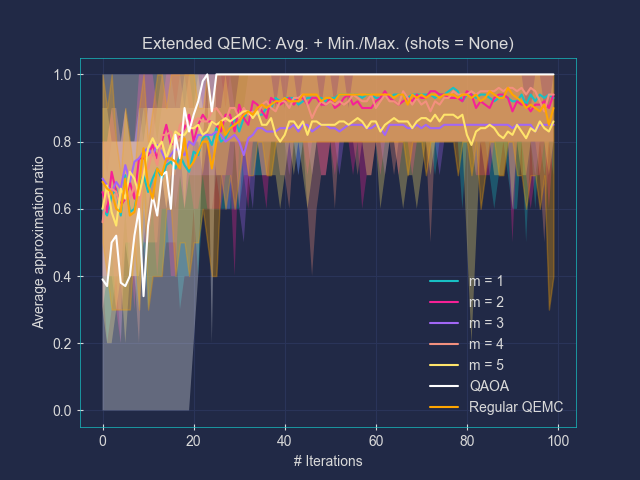
\includegraphics[width=1\textwidth]{Figures/Chapter_5/Extended-QEMC/8-node(n_layers=3, step_size=0.95, m=All).png}
    \caption{Implementation of the Unmodified Extended-\acrshort{qemc} scheme for the usual $8$-node graph: comparison with \acrshort{qaoa} and regular \acrshort{qemc} for various values of $m$. Note that $m$ is not extended beyond $5$, as this would exceed the number of qubits used in \acrshort{qaoa}}
    \label{fig:Vanilla_Extended-QEMC}
\end{figure}

As shown in the previous figure, the performance of the unmodified Extended-QEMC scheme is qualitatively very similar to that of regular QEMC. For some values of $m$, we achieve slightly better results, but these improvements are not particularly significant. After conducting several tests, I found no clear pattern to predict which values of $m$ would yield the best results, supporting the earlier conclusion. Therefore, this presents another heuristic for mapping the basis states, with performance comparable to the standard QEMC scheme. While this is a satisfactory outcome, it is not particularly remarkable.

%%%%%%%%%%%%%%%%%%%%%%%%%%%%%%%%%%%%%%%%%%%%%%%%%%%%%%%%%%%%%%%%%%%%%%%%
\protect\subsection{Cardinality \texorpdfstring{$= 1$}{= 1} Extended-QEMC}
\label{subsection:Card._eq_1_Extended_QEMC}

Motivated by the results in Figure \ref{fig:seed=13}\footnote{The trajectory of this study was far from linear. The results presented here are not in the chronological order of our research, hence this reference to later work, which was actually conducted before devising the Extended-QEMC scheme.}, I decided to make a slight change to the Unmodified Extended-\acrshort{qemc} scheme: instead of assigning $2^m$ basis states to each node, we assign only one basis state to each node (Cardinality $= 1$ Extended-\acrshort{qemc}). Although this adjustment occasionally yielded marginally better results than regular \acrshort{qemc}, we do not consider these improvements significant (see Figure \ref{fig:Card.=1_Extended-QEMC} for reference).
\begin{figure}[h]
    \centering
    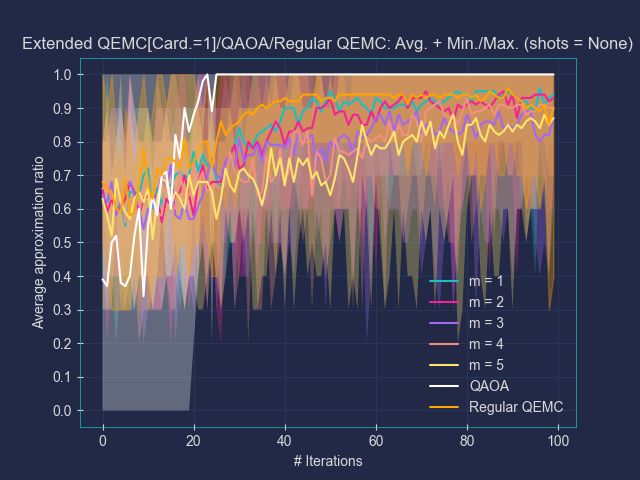
\includegraphics[width=1\textwidth]{Figures/Chapter_5/Extended-QEMC/8-node[Card.=1](n_layers=3, step_size=0.95, m=All).png}
    \caption{Implementation of the Cardinality $= 1$ Extended-\acrshort{qemc} scheme for the standard $8$-node graph: comparison with \acrshort{qaoa} and regular \acrshort{qemc} for various values of $m$.}
    \label{fig:Card.=1_Extended-QEMC}
\end{figure}

%%%%%%%%%%%%%%%%%%%%%%%%%%%%%%%%%%%%%%%%%%%%%%%%%%%%%%%%%%%%%%%%%%%%%%%%
\section{Alternative Ansätze}
\label{section:Alternative_ansätze}

After some reflection, I began to question whether the performance of \acrshort{qemc} and \acrshort{iqaqe} could be hindered by the use of a problem-agnostic ansatz. It's generally advantageous to incorporate problem-specific information into the ansatz, as exemplified by problem-inspired ansätze. Additionally, I pondered whether excessive entanglement or correlations among the system's basis states might be affecting the ansatz's performance. Such phenomena could make it challenging for the model to adjust the amplitude of a specific basis state without significantly impacting others. To address this potential issue, the concept of implementing non-deterministic CNOT gates (\acrshort{ndcnot}\textcolor{gray}{s}) occurred to me. This approach would allow the model to dynamically adjust the degree of entanglement. The most rudimentary way to implement this is by employing parameterized $R_x$ gates before each CNOT's control qubit, which is precisely what we did. The $R_x$ gate allows the control qubit to rotate in and out of the $\ket{1}$ state, thus adjusting the degree of entanglement introduced by the CNOT gate. The results for the standard $8$-node graph are presented below (Figure \ref{fig:ND-CNOTs}), for both \acrshort{qemc} and Cardinality $= 1$ Extended-\acrshort{qemc}.
\begin{figure}[h]
  \centering
  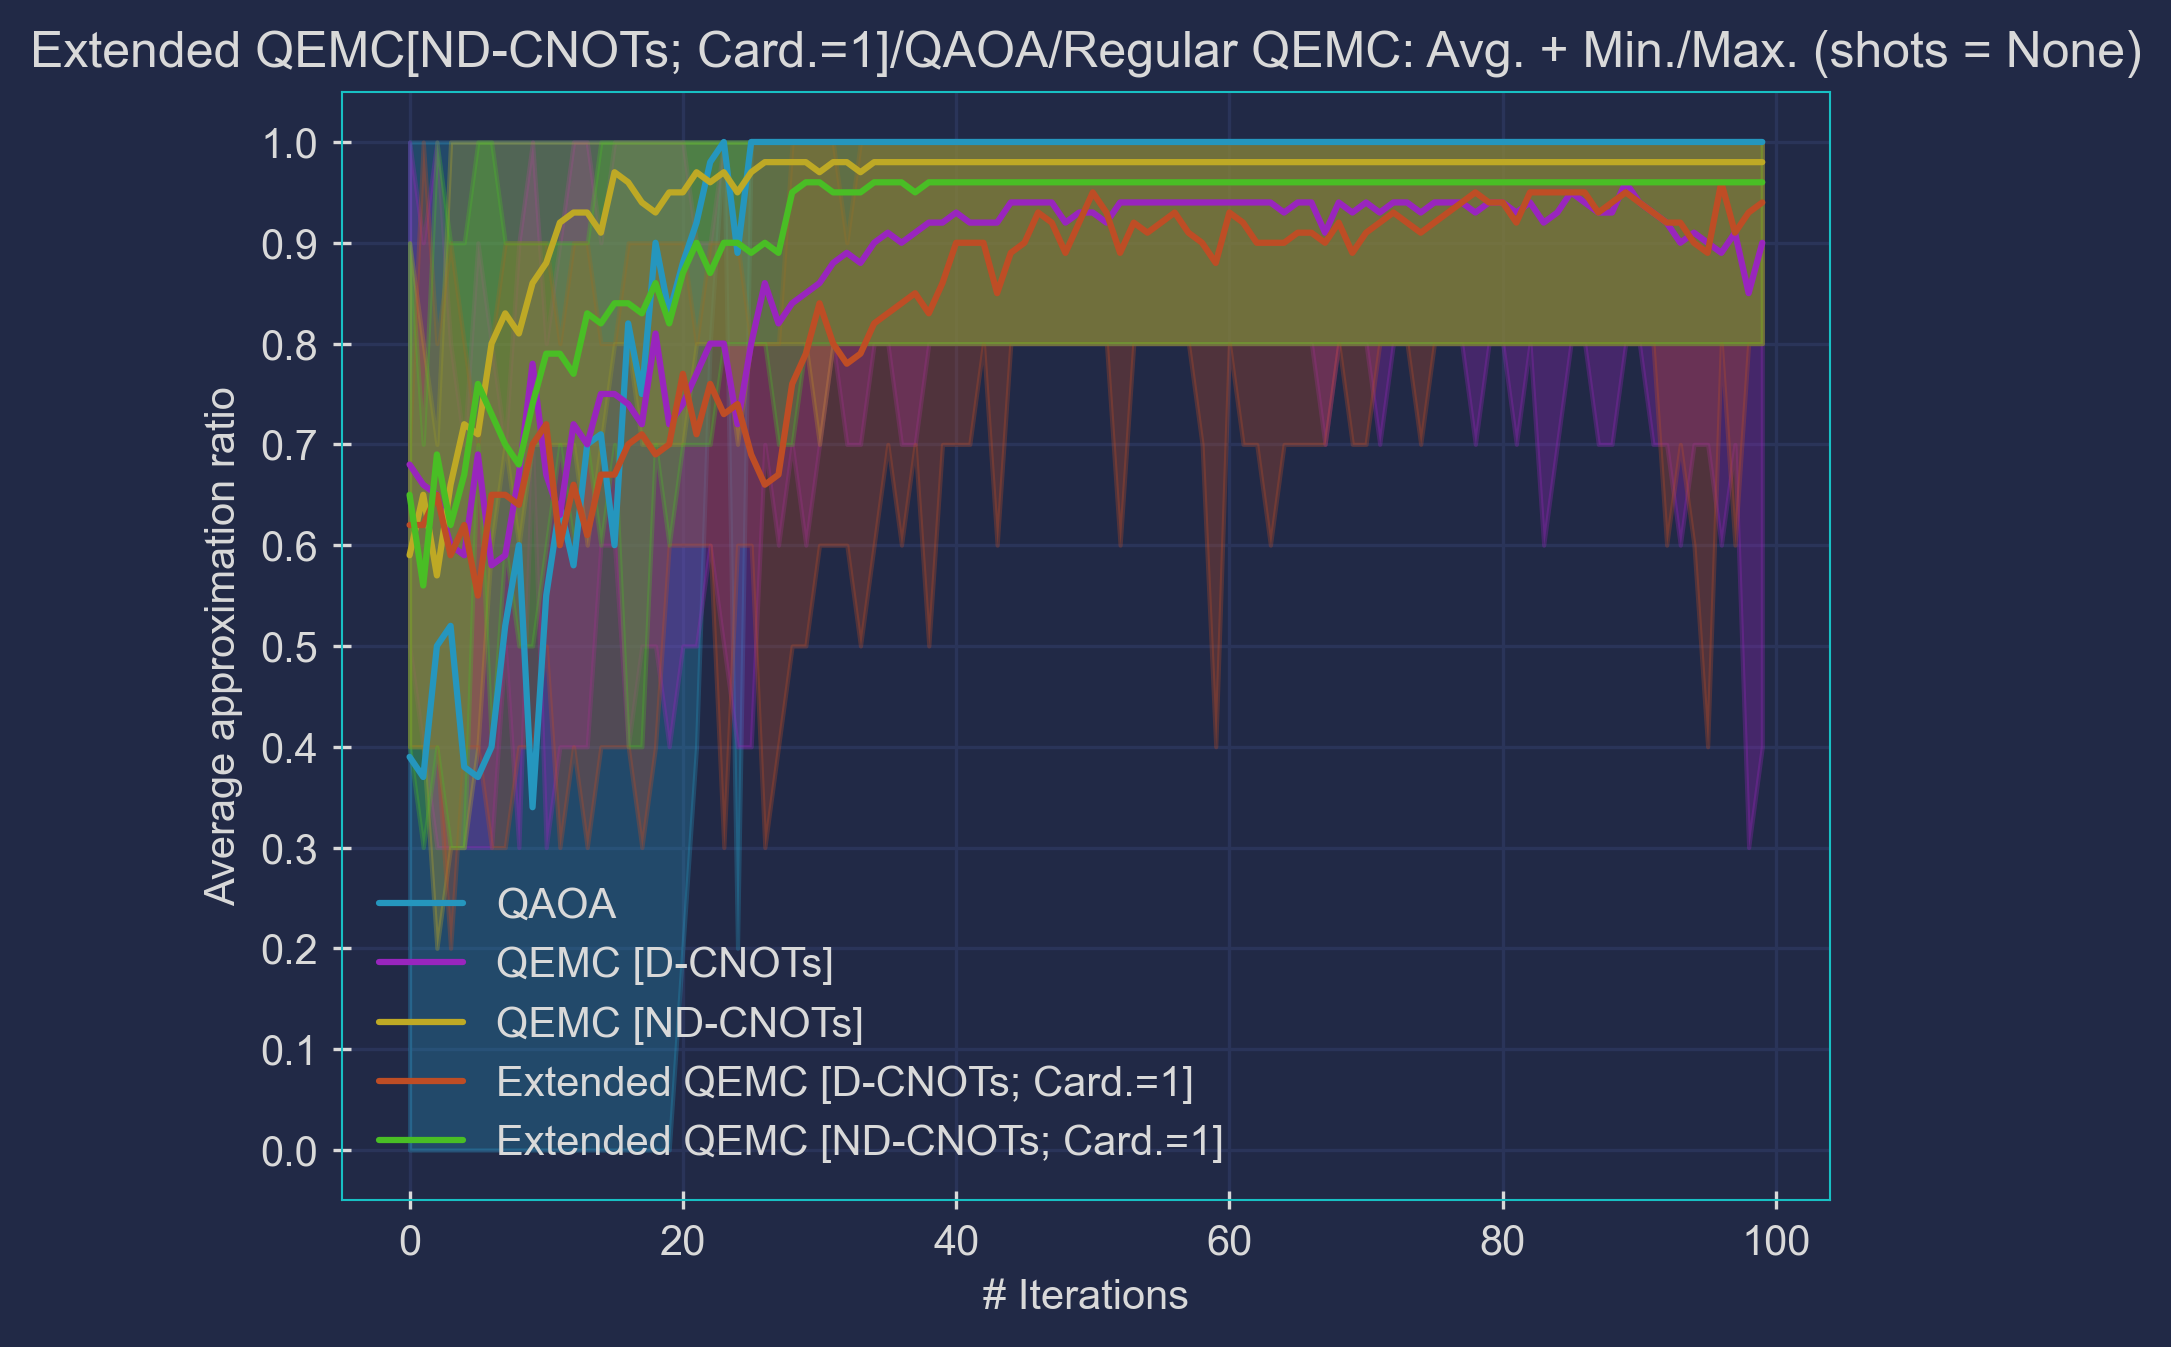
\includegraphics[width=1.0\textwidth]{Figures/Chapter_5/Extended-QEMC/8-node[ND-CNOTs; Card.=1](n_layers=2, step_size=0.5).png}
  \caption{Comparison of \acrshort{qemc} and Extended-\acrshort{qemc} implementations utilizing both \acrshort{dcnot}\textcolor{gray}{s} and \acrshort{ndcnot}\textcolor{gray}{s} for the usual $8$-node graph, alongside \acrshort{qaoa}.}
  \label{fig:ND-CNOTs}
\end{figure}

Several noteworthy observations can be made here. Firstly, it's apparent that \acrshort{ndcnot}-based schemes exhibit significantly more stable performance with fewer fluctuations compared to \acrshort{dcnot}-based schemes. This discrepancy arises from differences in their implementations: \acrshort{dcnot} circuits employ \texttt{n\_layers = 3} and a \texttt{step\_size = 0.95} (Adam's learning rate), whereas \acrshort{ndcnot} circuits use \texttt{n\_layers = 2} and \texttt{step\_size = 0.5}. The latter, \texttt{step\_size = 0.5}, accounts for the smoother curves observed in Figure \ref{fig:ND-CNOTs}, as expected, and may also contribute to faster convergence. Secondly, the performance appears noticeably enhanced when utilizing \acrshort{ndcnot}\textcolor{gray}{s}, particularly evident in the case of regular \acrshort{qemc}: a distinct improvement is evident when comparing the yellow and purple lines. Despite introducing added complexity to the optimization landscape, this approach appears to yield significant performance gains, at least for this small $8$-node graph. Thus, we've proposed a novel scheme that builds upon \acrshort{qemc}, showing great potential to outperform it.

Moreover, this analysis serves to validate the notion that deviating from purely problem-agnostic Ansätze is generally beneficial. This insight will inform our approach in developing future schemes in subsequent research endeavors. Encouraged by the promising outcomes from this study, we opted to expand the testing of this scheme to larger graphs to assess its scalability. Additionally, this paves the way for comparisons with the Goemans-Williamson scheme.





%%%%%%%%%%%%%%%%%%%%%%%%%%%%%%%%%%%%%%%%%%%%%%%%%%%%%%%%%%%%%%%%%%%%%%%%
\section{Goemans-Williamson and Bigger Graphs}
\label{section:GW_Bigger_Graphs}

At one point, I began to question whether it was appropriate to directly compare our results to \acrshort{qaoa}, which stands out as the best-performing \acrshort{vqa} among those tested. After thorough deliberation, we concluded that, indeed, it makes sense to do so for smaller graphs. However, as graphs increase in size, the availability of quantum machines with a necessary number of qubits to support such \acrshort{qaoa}\textcolor{gray}{s} becomes limited. This circumstance has led to the emergence of schemes like \acrshort{qemc} \cite{tenecohen2023variational} and others \cite{sciorilli2024largescale}, which aim to address the limitation imposed by the number of qubits.

In light of this, I proceeded to evaluate the performance of our proposed schemes on significantly larger graphs. Two such graphs were considered:
\begin{enumerate}
    \item $32$-node Erdős–Rényi graph, constructed using NetworkX's {\hypersetup{urlcolor=black}\url{nx.erdos\_renyi\_graph(n = 32, p = 0.2, seed=0, directed=False)}}, where each edge is included in the graph with a probability of $p = 0.2$;
    \item $100$-node Erdős–Rényi graph, defined similarly to the previous graph, utilizing {\hypersetup{urlcolor=black}\url{nx.erdos\_renyi\_graph(n = 100, p = 0.2, seed=0, directed=False)}}.
\end{enumerate}
The results obtained from these evaluations are presented below\footnote{Please note that we have included only the most promising schemes.} (Figures \ref{fig:32-node_Graph(2-Subfigures)} and \ref{fig:100-node_Graph(2-Subfigures)}).

\begin{figure*}[hb!]
    \centering
    \begin{subfigure}[b]{0.495\textwidth}
        \centering
        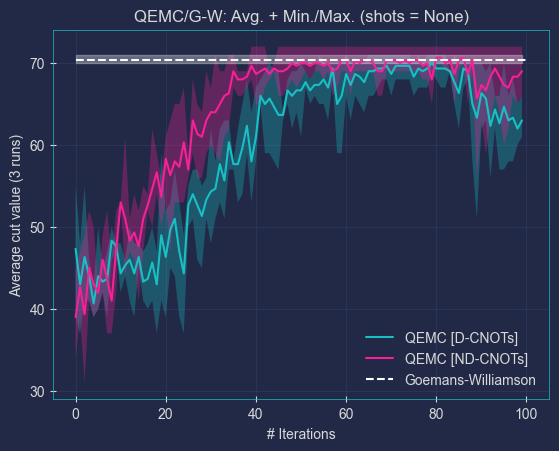
\includegraphics[width=1\textwidth]{Figures/Chapter_5/Large graphs/32-node_Graph(QEMC&G-W).png}
        \caption{$32$-node graph – \acrshort{qemc} and \acrshort{gw} exclusively.}
        \label{fig:32-node_Graph(QEMC&G-W)}
    \end{subfigure}
    \hfill
    \begin{subfigure}[b]{0.495\textwidth}
        \centering
        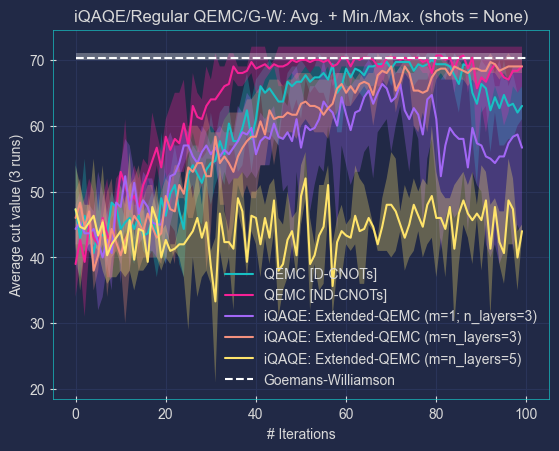
\includegraphics[width=1\textwidth]{Figures/Chapter_5/Large graphs/32-node_Graph.png}
        \caption{$32$-node graph – other schemes.}
        \label{fig:32-node_Graph}
    \end{subfigure}
    \caption{Comparison of performance (average cut values) among various \acrshort{vqa} schemes for the specified $32$-node graph. \texttt{n\_layers = 3} was employed for both \acrshort{qemc}\textcolor{gray}{s}, with \texttt{step\_size = 0.95} for \acrshort{dcnot}-\acrshort{qemc} and \texttt{step\_size = 0.5} for \acrshort{ndcnot}-\acrshort{qemc}. For all Extended-\acrshort{qemc} schemes, a \texttt{step\_size = 0.95} was utilized, with the number of layers specified in the legend.}
    \label{fig:32-node_Graph(2-Subfigures)}
\end{figure*}

\clearpage

\begin{figure*}[hb!]
    \centering
    \begin{subfigure}[b]{0.495\textwidth}
        \centering
        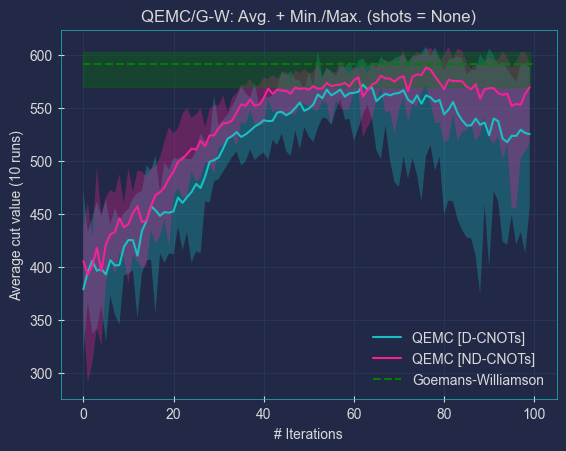
\includegraphics[width=1\textwidth]{Figures/Chapter_5/Large graphs/100-node_Graph(QEMC&G-W).png}
        \caption{$100$-node graph – \acrshort{qemc} and \acrshort{gw} exclusively.}
        \label{fig:100-node_Graph(QEMC&G-W)}
    \end{subfigure}
    \hfill
    \begin{subfigure}[b]{0.495\textwidth}
        \centering
        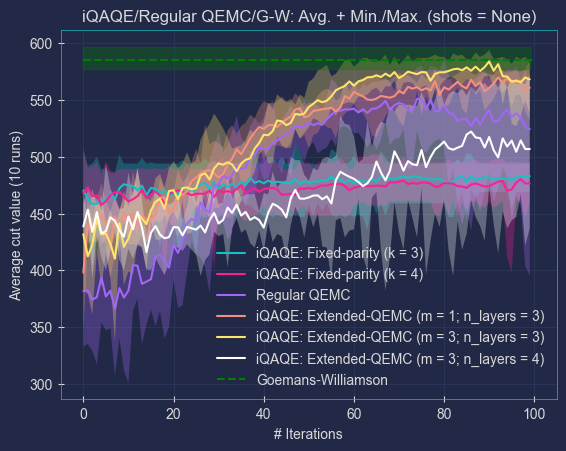
\includegraphics[width=1\textwidth]{Figures/Chapter_5/Large graphs/100-node_Graph.png}
        \caption{$100$-node graph – other schemes.}
        \label{fig:100-node_Graph}
    \end{subfigure}
    \caption{Comparison of performance (average cut values) among various \acrshort{vqa} schemes for the specified $100$-node graph. This time, all considered VQAs utilized \texttt{n\_layers = 3} and \texttt{step\_size = 0.95}, except for Extended-\acrshort{qemc} with $m=3$, which used \texttt{n\_layers = 4}.}
    \label{fig:100-node_Graph(2-Subfigures)}
\end{figure*}
% Notice how I added Fixed-parity iQAQE to Fig. 5.16 (b). Say this in the text, somewhere.

% Re-read this part!
In Figure \ref{fig:100-node_Graph(2-Subfigures)}, note that \acrshort{qemc}, fixed-parity \acrshort{iqaqe}, and \acrshort{gw} employ $10$ runs for averaging, while all other schemes (including Cardinality $= 1$ Extended-\acrshort{qemc}) use only $5$ runs. This decision was made to expedite the process while ensuring reasonable averaging of statistical fluctuations in the results. Likewise, in Figure \ref{fig:32-node_Graph(2-Subfigures)}, only $3$ runs were utilized for all schemes. Additionally, in Figure \ref{fig:100-node_Graph(2-Subfigures)}, I chose to include the fixed-parity \acrshort{iqaqe} scheme to evaluate its performance on a larger graph.

Now, concerning the results, several interesting observations emerge. For the $32$-node graph, Extended-\acrshort{qemc}'s performance varies considerably with different values of $m$ and \texttt{n\_layers}, as previously observed, making it inconsistent and challenging to optimize for other graphs. Once again, we observe the benefits of using \acrshort{ndcnot}\textcolor{gray}{s} in \acrshort{qemc} compared to the usual \acrshort{dcnot}\textcolor{gray}{s}. Although the average performances have not yet reached the level of the Goemans-Williamson algorithm, indicated by the white dashed line in Figure \ref{fig:32-node_Graph}, the maximum performances achieved by the \acrshort{ndcnot}-based scheme surpass the best performance attained by \acrshort{gw}, as evident from the comparison of the shaded pink and white regions. This marks the first instance in this study where one of our heuristics surpasses classical state-of-the-art algorithms, representing a significant milestone and underscoring the potential for further exploration of the proposed \acrshort{iqaqe} Framework.

Turning to the $100$-node graph, similar trends are observed across the board. Additionally, we observed that the previously mentioned fixed-parity \acrshort{iqaqe} performs exceptionally poorly, indicating its inability to generalize for larger graphs. Nevertheless, as with the $32$-node graph, reaching the performance level of the Goemans-Williamson algorithm on average remains elusive, indicating ample room for improvement. However, once again, promising results are seen in the maximum cuts (shaded regions).






%%%%%%%%%%%%%%%%%%%%%%%%%%%%%%%%%%%%%%%%%%%%%%%%%%%%%%%%%%%%%%%%%%%%%%%%
\section{Average Best-so-Far correction}
\label{section:Avg_BSF_correction}

% Average Best-so-Far correction and its results. Mention how it was "wrong", initially, and how it was "fixed". I'm not sure where to include this, though.

% I think I should send these plots to an Appendix, so I can save some space.

As previously noted, there exists a distinction between implementing the \acrshort{bsf} transformation before and after the averaging process. We assert that the former (prior to averaging) provides the most accurate representation of the algorithm's optimal performance. Therefore, in alignment with the average \acrshort{ar} plots previously showcased, we opted to rerun several earlier schemes with the \acrshort{bsf} transformation applied before averaging. Given the substantial number of resulting graphs, they will be included in Appendix \ref{appendix:BSF_correction}.

% Maybe, include only the $100$-node graph's results here, and send the rest to the Appendix. I've re-run this! It's in 'Avg._BSF_Correction.ipynb', near the end of the notebook. (In case I decide to include this here.)





%%%%%%%%%%%%%%%%%%%%%%%%%%%%%%%%%%%%%%%%%%%%%%%%%%%%%%%%%%%%%%%%%%%%%%%%
\section{Randomized iQAQE benchmarking}
\label{section:Randomized_iQAQE_benchmarking}

In this section, our aim is to adopt a more systematic approach to identify ways to enhance the mapping of basis states. While heuristics have served us thus far, we sought to determine whether there are additional patterns that we may have overlooked by relying solely on these heuristics.

% Talk about the randomized benchmarking that we've been doing, and how it's been helping us to understand the performance of the different schemes. Type $1$ and $2$ variables, etc. This could have many subsections.

\subsection*{Initial proposition}
Continuing from the earlier discussion, we ran numerous \acrshort{iqaqe} instances, each with random qubit number, list cardinalities and assignments\footnote{We always employed \texttt{n\_layers = 3} and \texttt{step\_size = 0.99}. This time, the final selected cut is derived from the \acrshort{bsf} average curve (not the average \acrshort{bsf}), constructed from $10$ repetitions. Although not optimal, this does not alter our interpretation of the results.}. The underlying idea was to identify optimal combinations of qubit number, list cardinalities and mapping by running multiple instances of \acrshort{iqaqe}. Subsequently, we aimed to discern meaningful patterns that could inform the development of a strategy for more refined basis state selection. However, our analysis did not yield a clear indication of how the partitioning should proceed. As demonstrated below, there existed a plethora of vastly different combinations of partitioning and list cardinality that performed similarly well. Consequently, it proved humanly impossible to extract any coherent insights from this dataset. The results supporting this claim are presented in Figure \ref{fig:Random_iQAQE(Seeds)} for the usual $8$-node graph.
\begin{figure*}[hb!]
  \centering
  \begin{subfigure}[t]{0.495\textwidth}
      \centering
      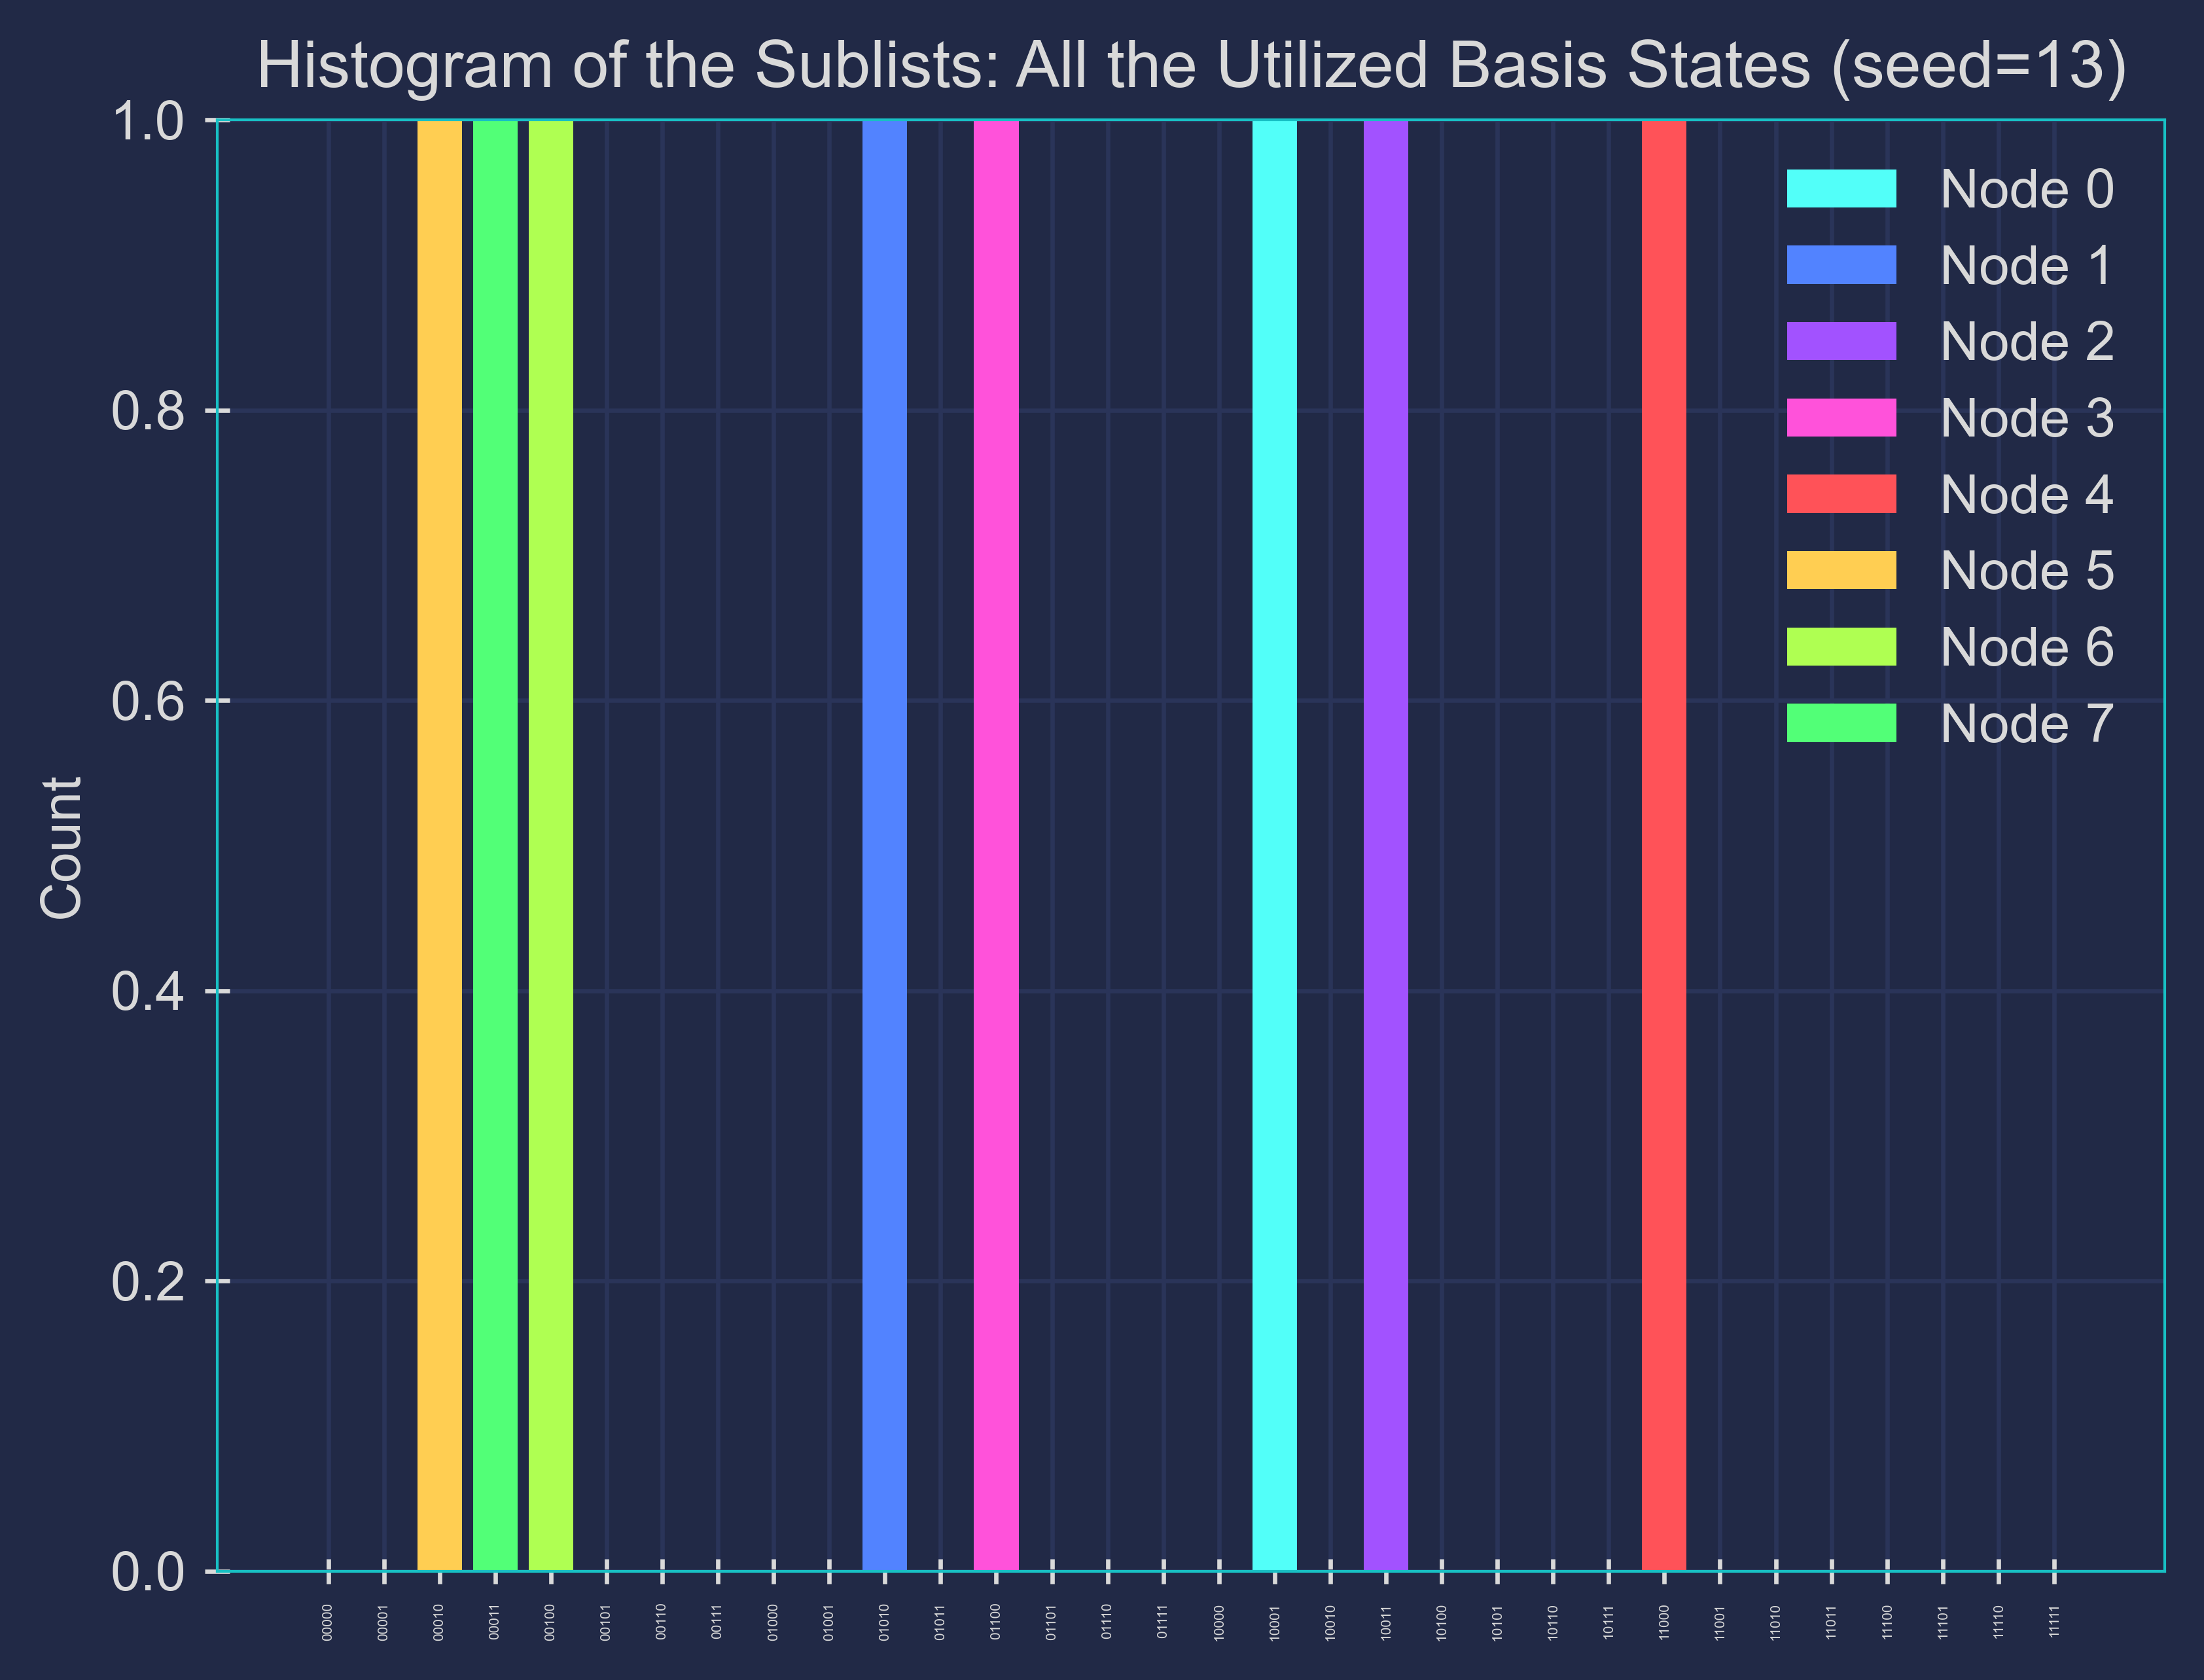
\includegraphics[width=1\textwidth,height=0.75\textwidth]{Figures/Chapter_5/Random iQAQE (Coloured plots)/8-node(seed=13).png}
      \caption{Seed = $13$.}
      \label{fig:seed=13}
  \end{subfigure}
  \hfill
  \begin{subfigure}[t]{0.495\textwidth}
      \centering
      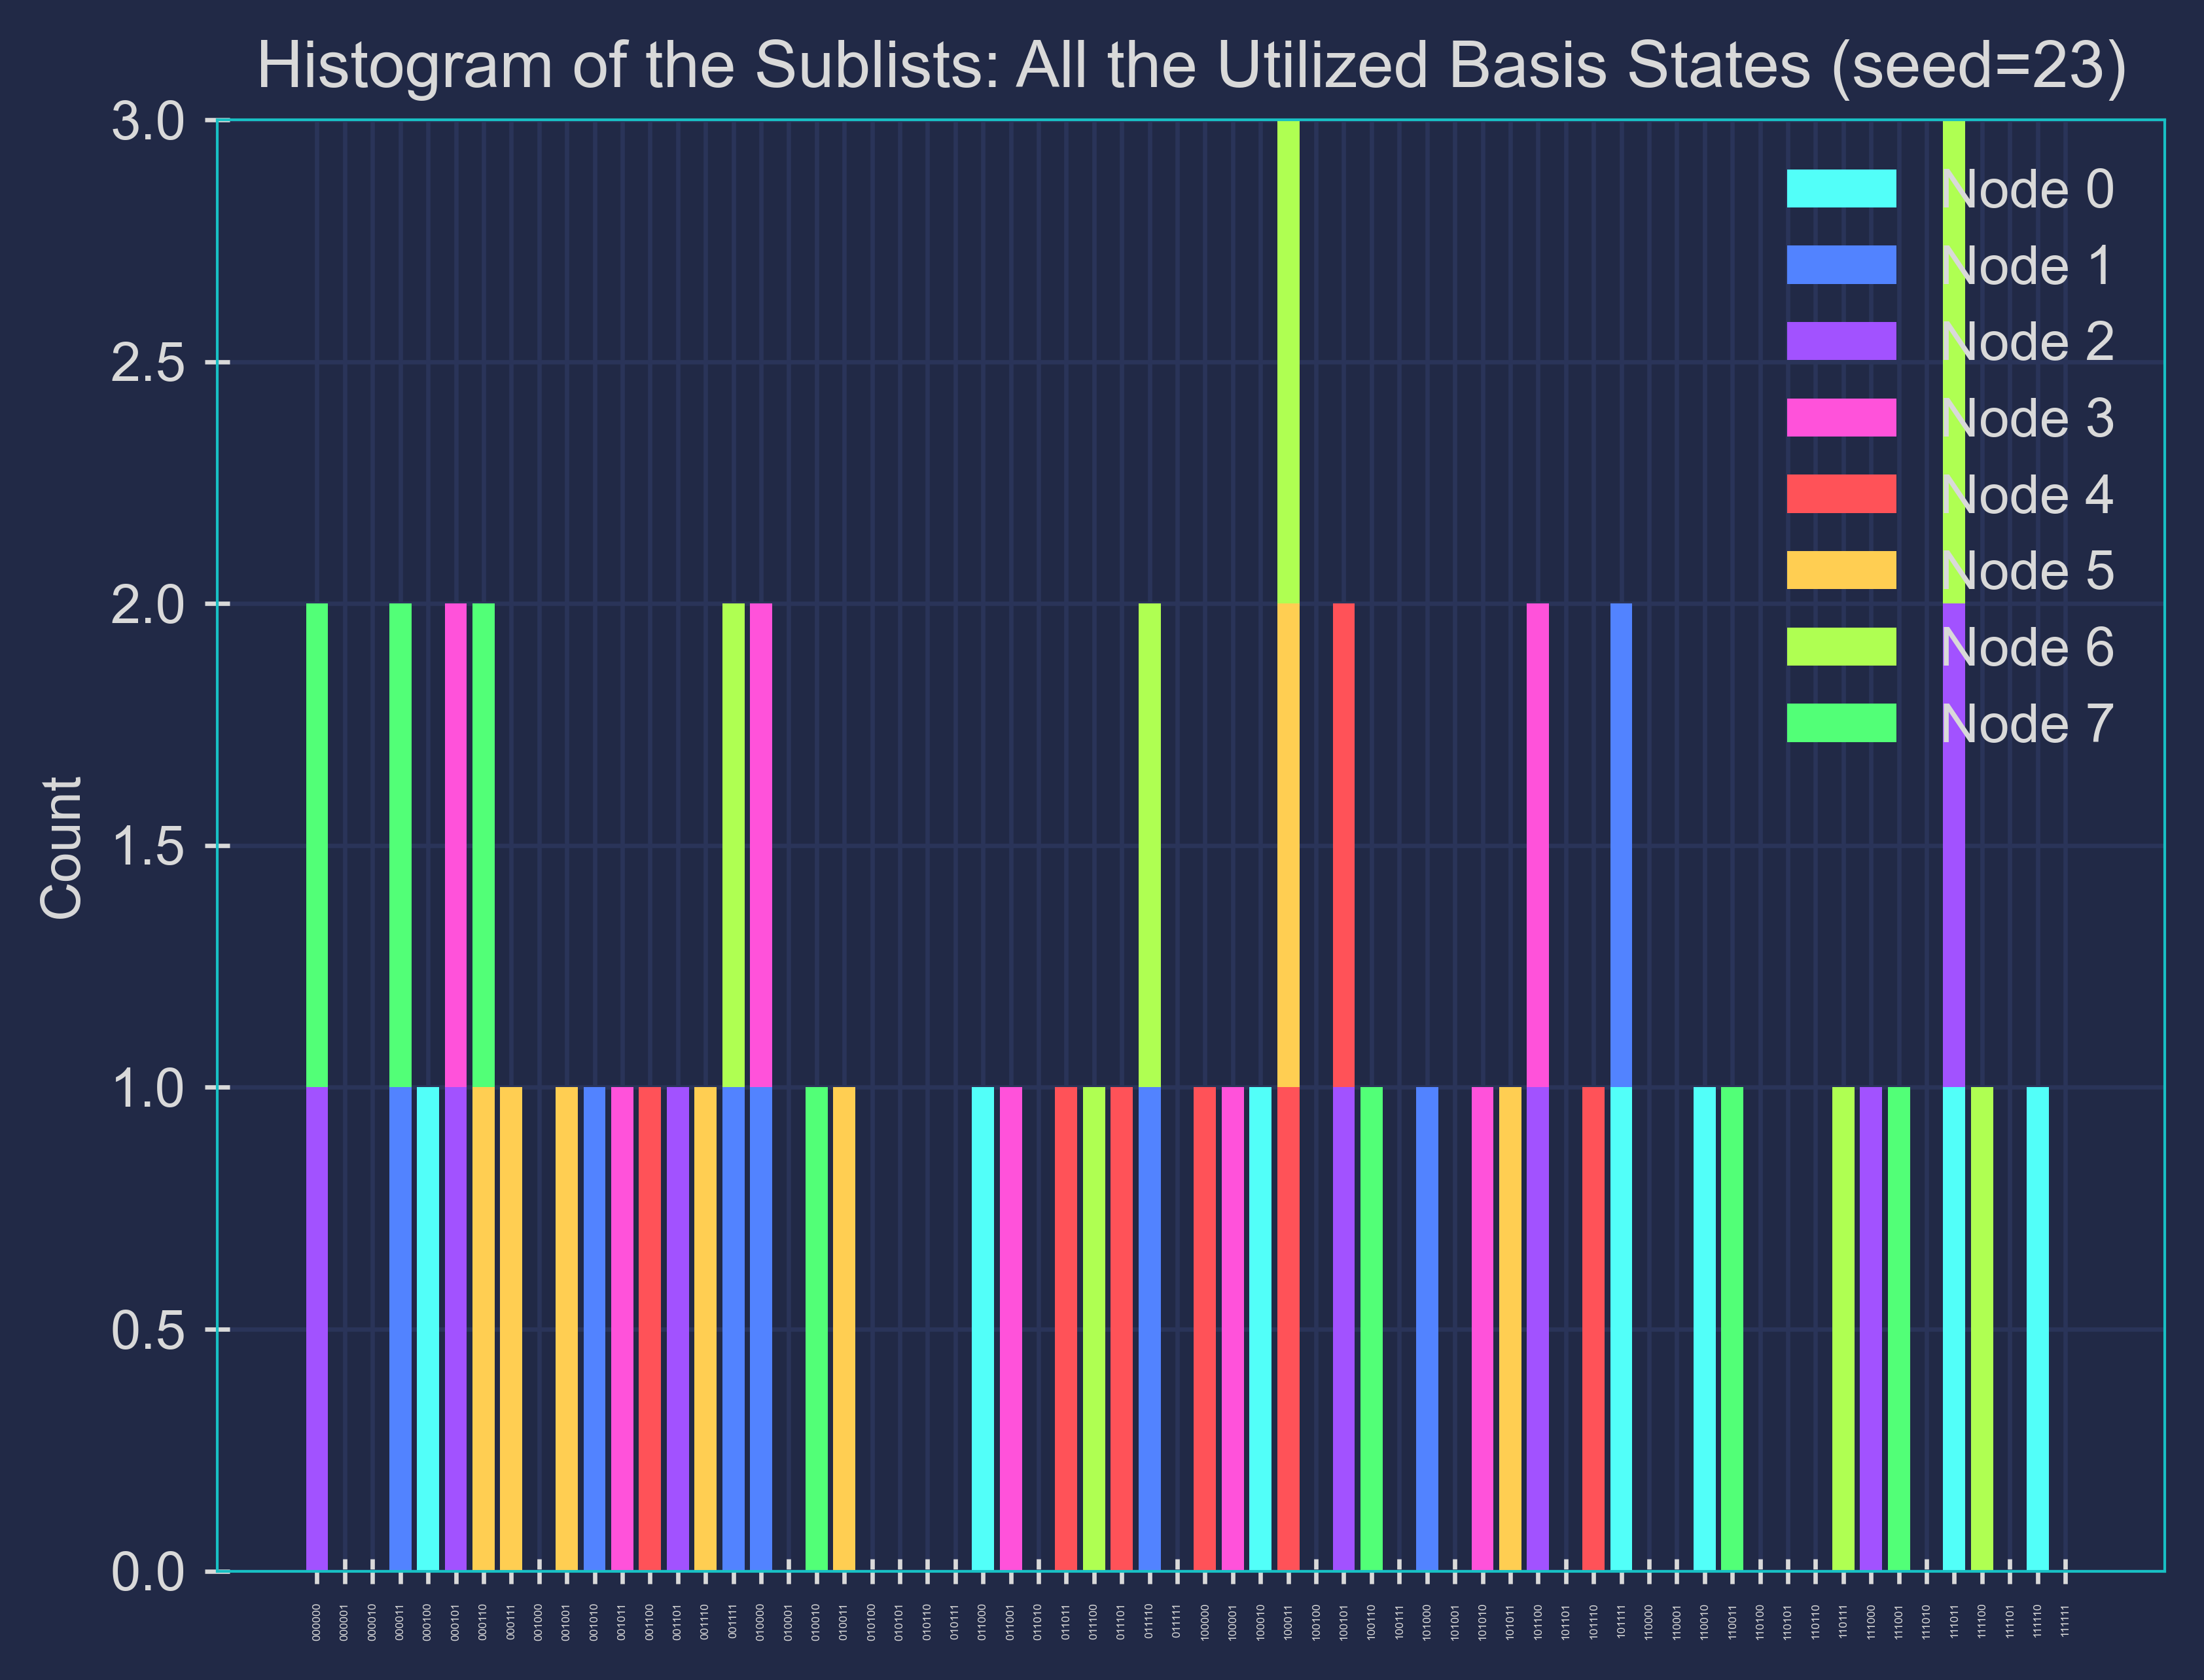
\includegraphics[width=1\textwidth,height=0.75\textwidth]{Figures/Chapter_5/Random iQAQE (Coloured plots)/8-node(seed=23).png}
      \caption{Seed = $23$.}
      \label{fig:seed=23}
  \end{subfigure}
\end{figure*}

% \bigskip

\clearpage

\begin{figure*}[ht!]
  \addtocounter{figure}{-1} % Added <<
  \centering
  \begin{subfigure}[t]{0.325\textwidth}
      \addtocounter{subfigure}{2} % Added <<
      \centering
      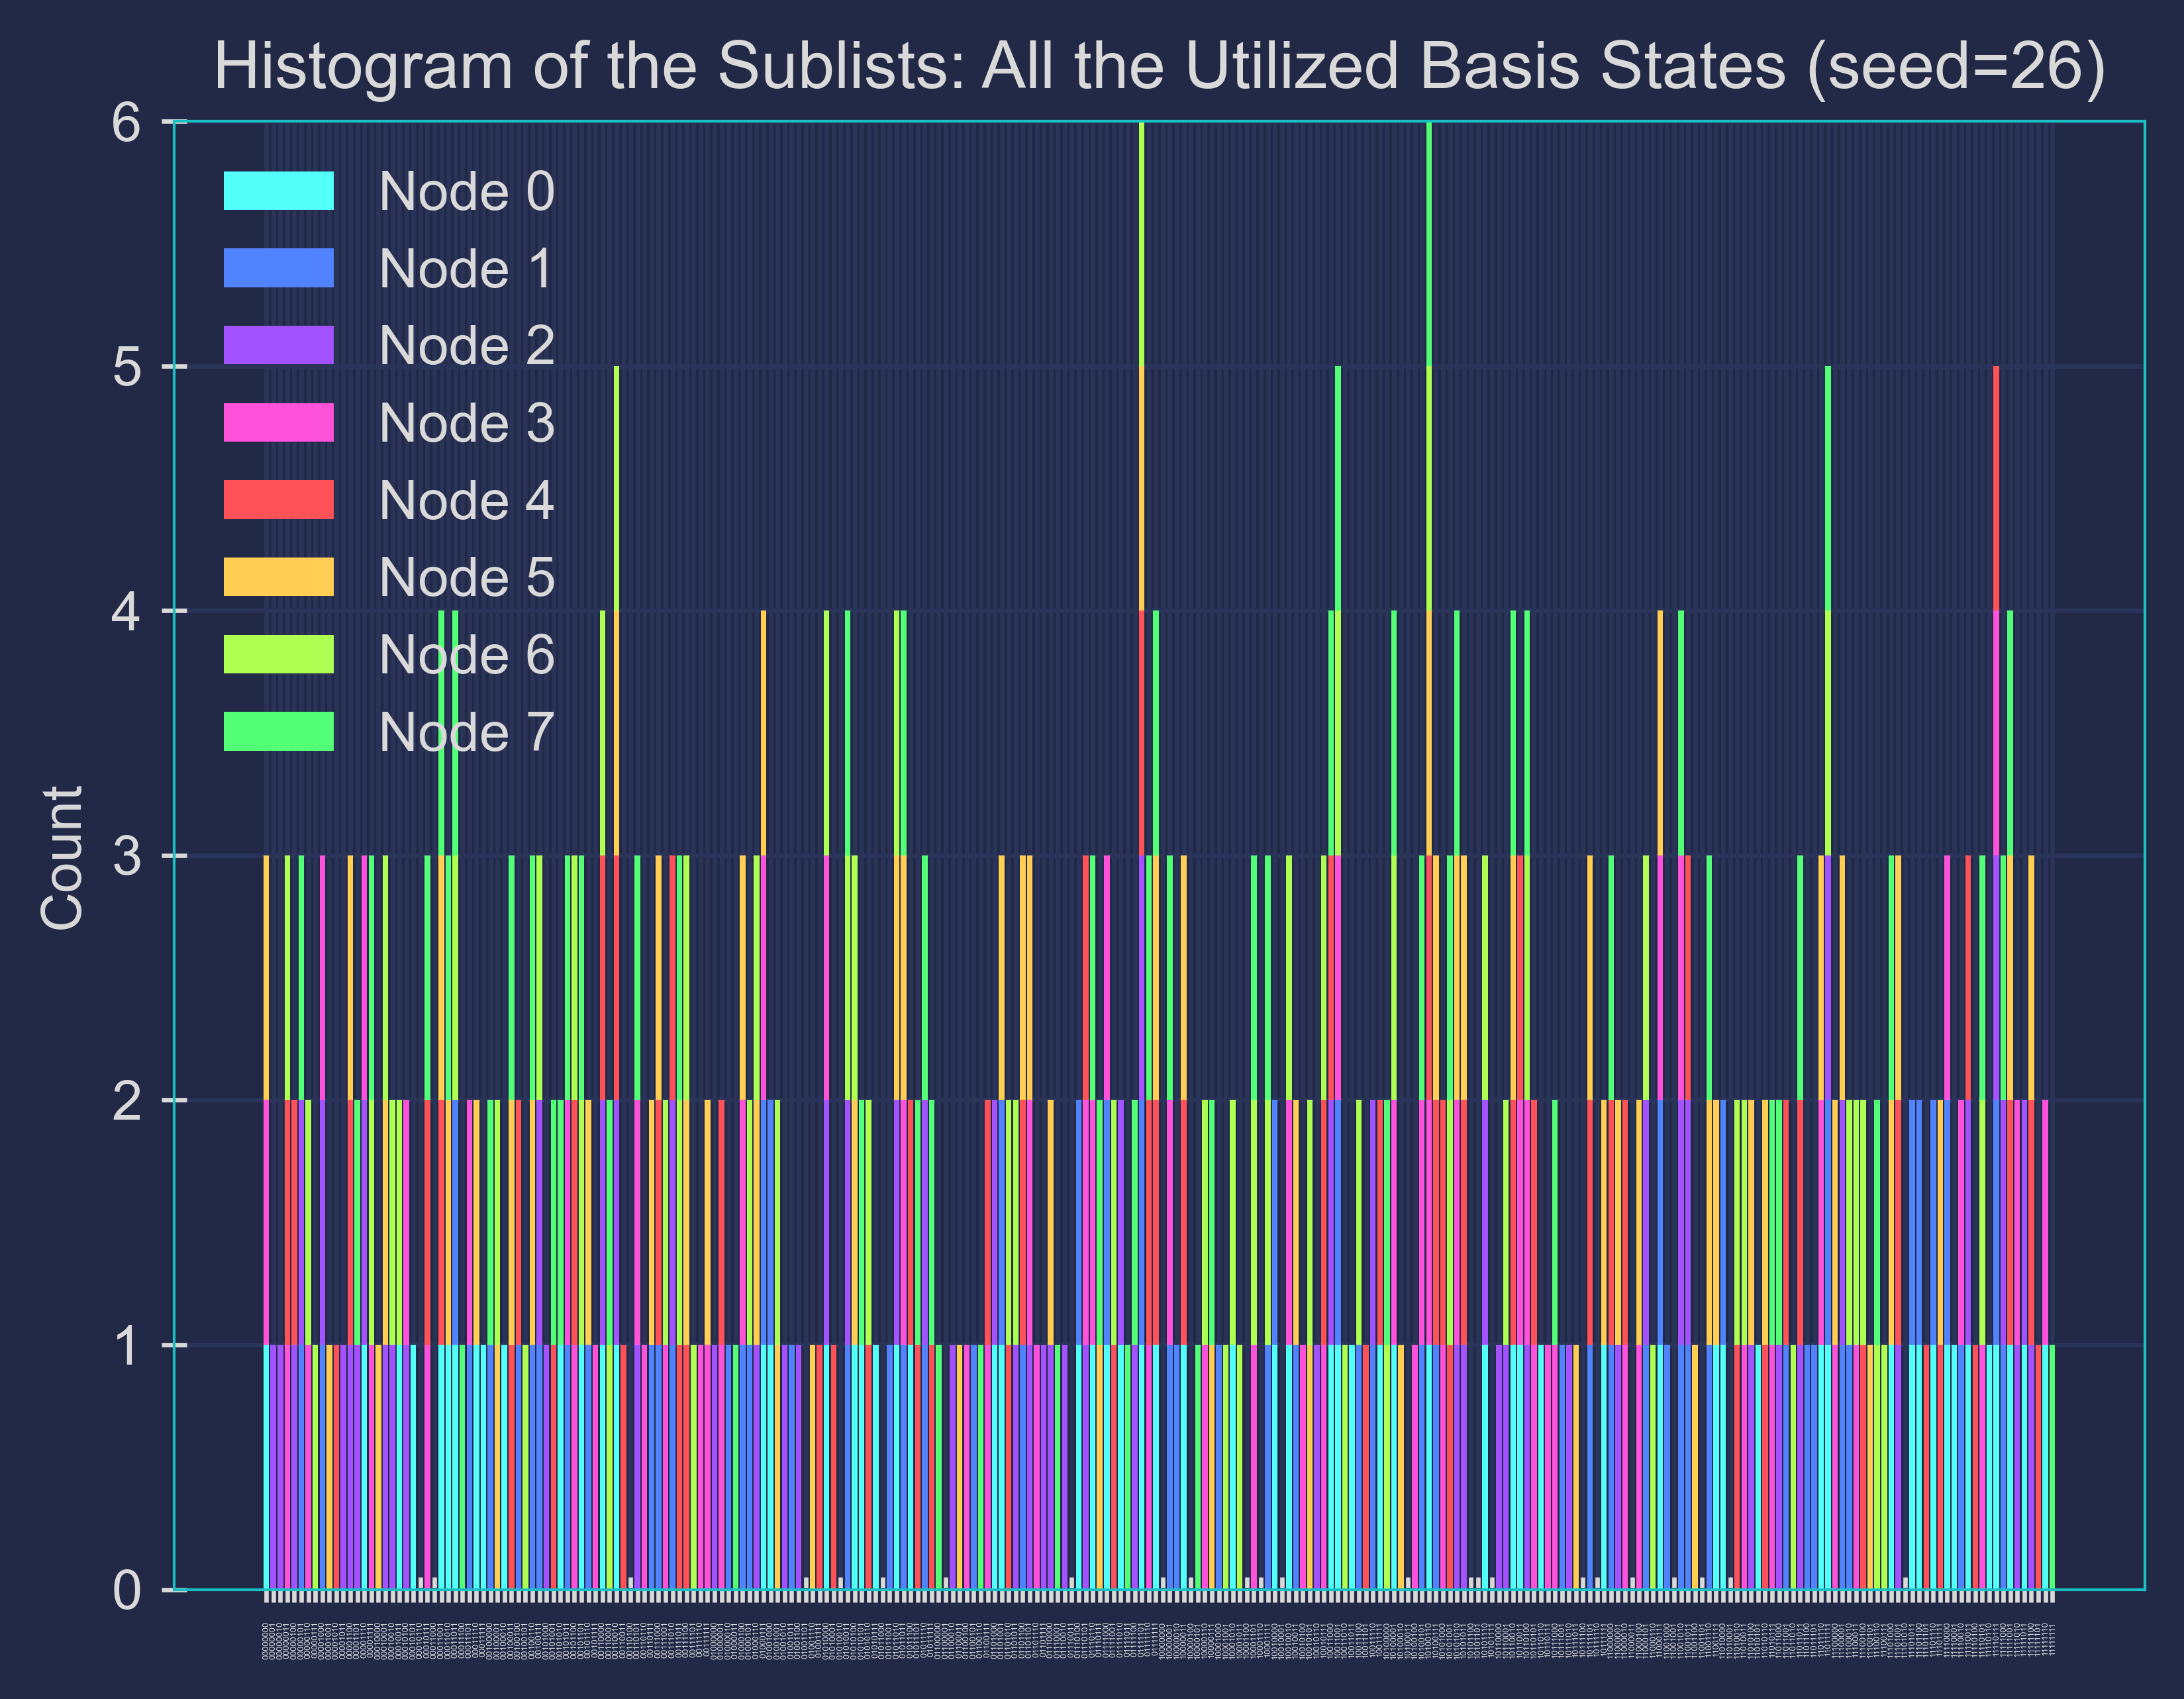
\includegraphics[width=1\textwidth,height=4.25cm]{Figures/Chapter_5/Random iQAQE (Coloured plots)/8-node(seed=26).png}
      \caption{Seed = $26$.}
      \label{fig:seed=26}
  \end{subfigure}
  \hfill
  \begin{subfigure}[t]{0.325\textwidth}
      \centering
      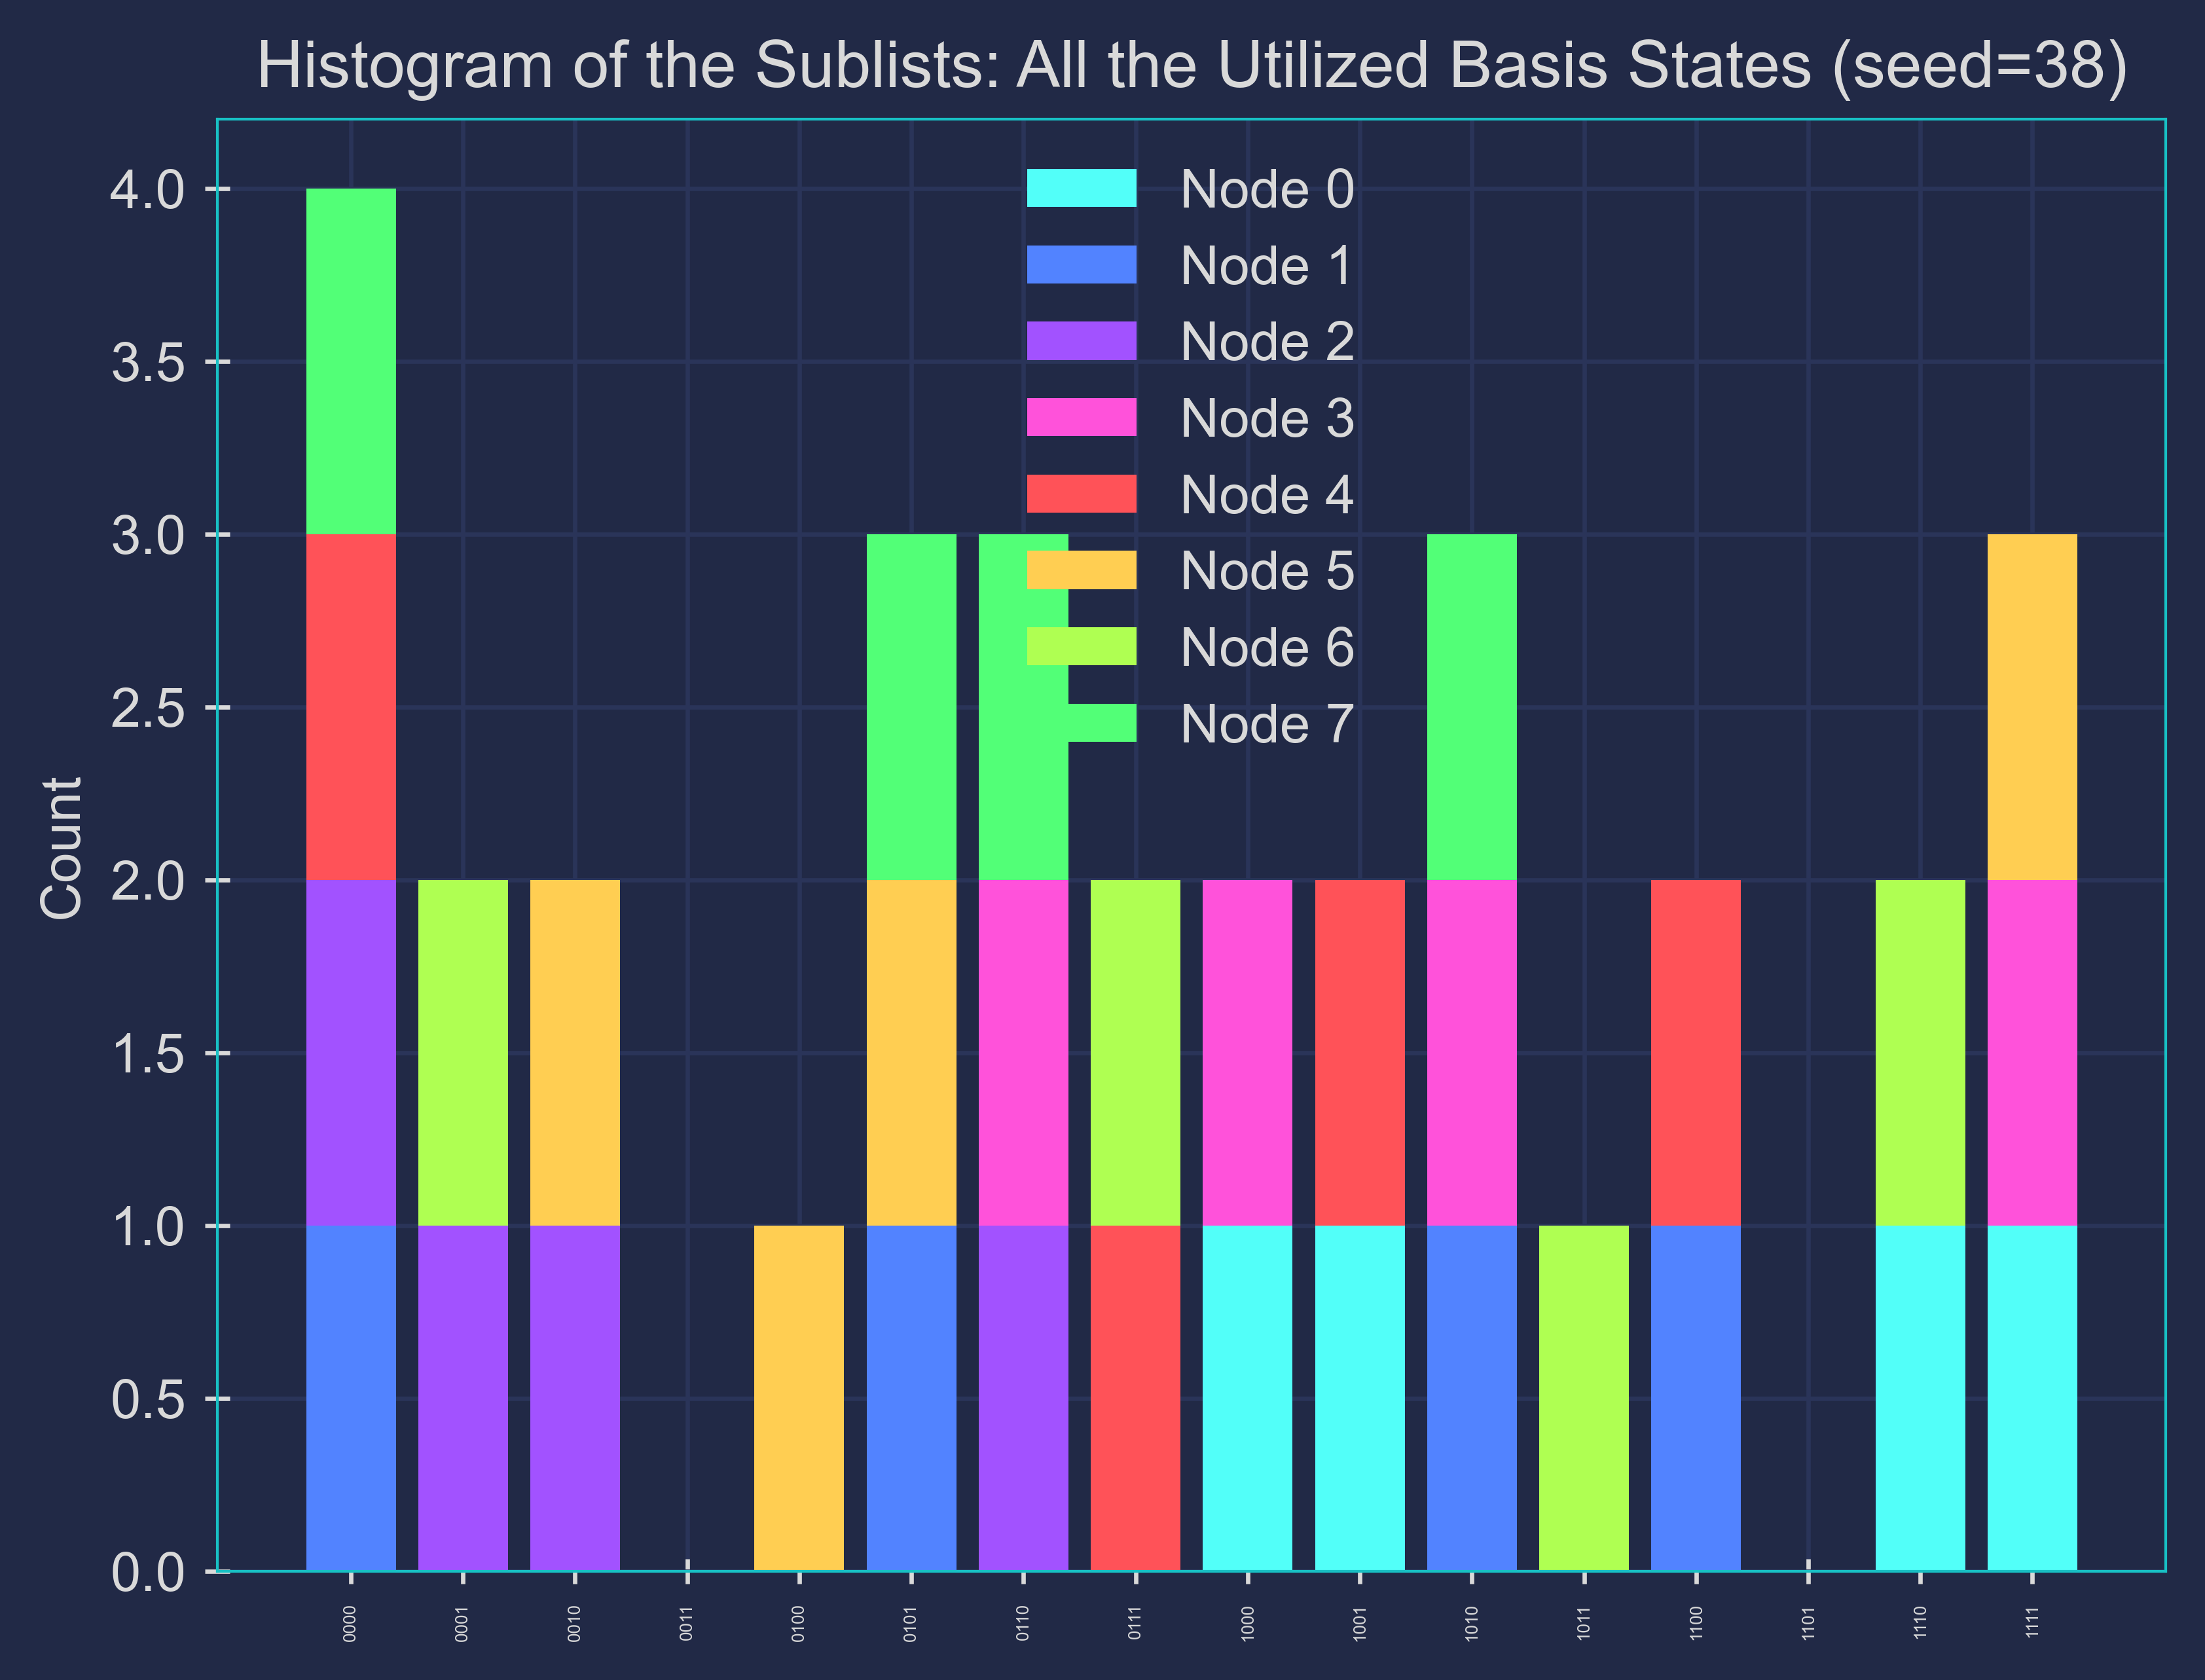
\includegraphics[width=1\textwidth,height=4.25cm]{Figures/Chapter_5/Random iQAQE (Coloured plots)/8-node(seed=38).png}
      \caption{Seed = $38$.}
      \label{fig:seed=38}
  \end{subfigure}
  \hfill
  \begin{subfigure}[t]{0.325\textwidth}
      \centering
      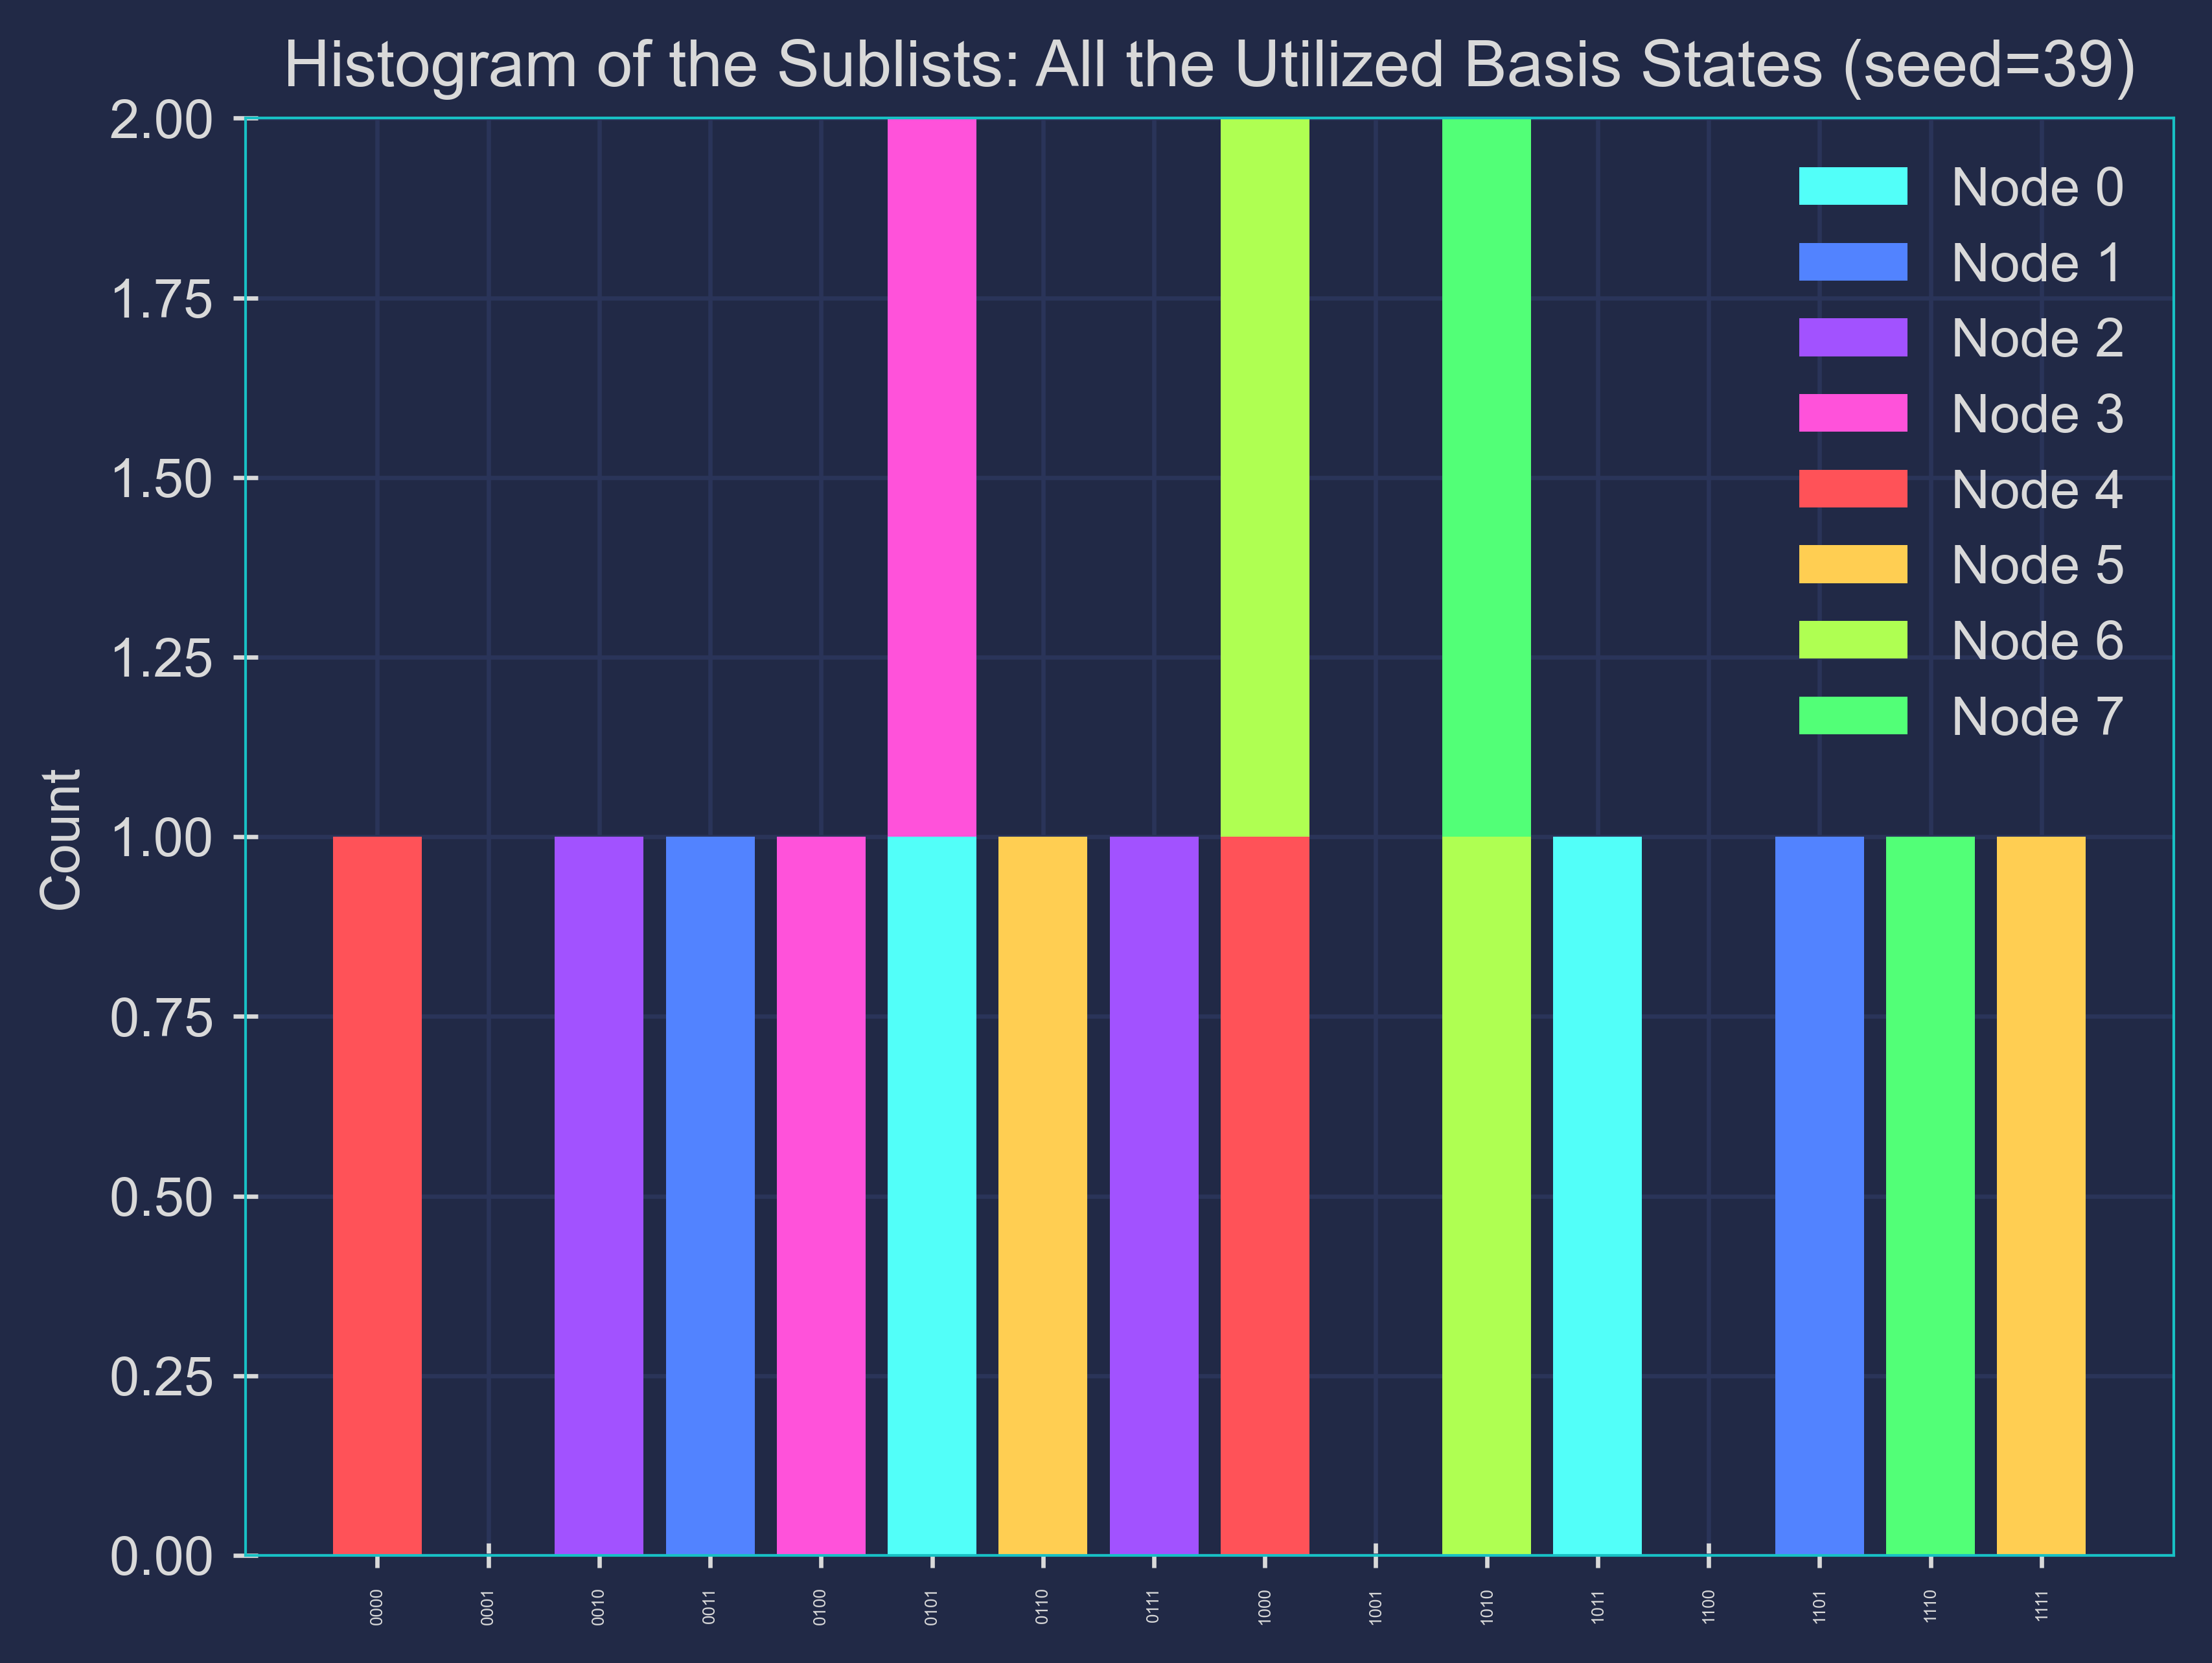
\includegraphics[width=1\textwidth,height=4.25cm]{Figures/Chapter_5/Random iQAQE (Coloured plots)/8-node(seed=39).png}
      \caption{Seed = $39$.}
      \label{fig:seed=39}
  \end{subfigure}
  \caption{Basis states' distributions over the $8$ nodes of the usual graph, for many different \texttt{np.random.seed} seeds. Only those for which the average best-so-far approximation ratio [after $100$ iQAQE iterations] was found to be $\geq 0.975$ were selected. (These were the best performing seeds out of the $50$ tested, for \texttt{seed} $\in \left[0, 49\right] \cap \mathbb{Z}$.)}
  \label{fig:Random_iQAQE(Seeds)}
\end{figure*}

As can be seen, not much can be directly inferred from this. When confronted with seemingly unstructured data, a natural progression is to employ machine learning schemes to discern patterns. Indeed, this aligns with the forte of such models. Various options were considered, spanning from neural networks to regression and clustering models. Initially, we opted to implement a basic regression model for its simplicity. Establishing such a model necessitates identifying a set of statistical properties of the input data (lists of basis states) that can serve as inputs for the regression model. This discussion follows in the subsequent section.

\subsection*{Machine learning-based approach}
Following the prior discussion regarding the \acrshort{iqaqe} formalism (refer to Figure \ref{fig:Random_iQAQE(Seeds)}), our objective was to construct a small machine learning (\acrshort{ml}) model aimed at comprehending the patterns in basis states' partitioning that contribute to the algorithm's performance variations. Naturally, such a model necessitates defining input (independent variables - \acrshort{iv}) and output (dependent variable - \acrshort{dv}). As previously mentioned, our \acrshort{iv}\textcolor{gray}{s} will encompass statistically significant properties extracted from each specific sub-list encoding. Alternatively, including the basis states' partitioning directly as the model's input presents challenges concerning memory-efficient encoding. Traditional one-hot encoding methods are inadequate due to the vast number of potential basis states available (which scales exponentially with the number of qubits). Thus, we opted for the following statistical properties:
\begin{itemize}
  \item {\large\textbf{Type $1$ variables}} - these are input variables that are defined for each of the sub-lists of basis states. They are:
  \begin{itemize}
      \item \textbf{Number of basis states} in each sub-list, the so-called cardinality of the sub-list;
      \item \textbf{Average Hamming weight} in each sub-list;
      \item \textbf{Standard deviation/variance of the Hamming weights} in each sub-list;
      \item \textbf{Average pair-wise Hamming distance} between the basis states in each sub-list;
      \item \textbf{Standard deviation/variance of the pair-wise Hamming distances} between the basis states in each sub-list;
      \item \textbf{Parity score} of each sub-list: this is obtained by: \#(Even basis states) $-$ \#(Odd basis states), for each sub-list.
  \end{itemize}
  \item {\large\textbf{Type $2$ variables}} - these are input variables that are defined for the entire set of basis states. They are:
  \begin{itemize}
      \item \textbf{Average Hamming weight} of the entire set of basis states;
      \item \textbf{Standard deviation/variance of the Hamming weights} of the entire set of basis states;
      \item \textbf{Average pair-wise Hamming distance} between the basis states in the entire set;
      \item \textbf{Standard deviation/variance of the pair-wise Hamming distances} between the basis states in the entire set;
      \item \textbf{Parity score} of the entire set of basis states. (Given by the sum of the parity scores of the sub-lists);
      \item \textbf{Global basis-states' entropy} [of the entire set of basis states]: this is given by the Shannon entropy of the basis states' distribution in the entire set. It is calculated as: $-\frac{1}{\log_2(N)}\sum_{i=1}^{N} p_i \log_2(p_i)$, where $p_i$ is the probability of the $i^{th}$ basis state in the entire set. Note that it is normalized by the maximum entropy value, which is $\log_2(N)$, where $N$ is the total number of basis states in the entire set. (This entropy's maximum is achieved when we have a uniform distribution of the basis states.) Also, this is a measure of the randomness of the basis states' distribution in the entire set.
  \end{itemize}
\end{itemize}
The dataset was constructed in a similar manner to that of Figure \ref{fig:Random_iQAQE(Seeds)}, but expanded to encompass $1000$ seeds. For each seed, we computed the \textbf{median} \acrshort{bsf} vector (\acrshort{dv}) and the associated independent variables (\acrshort{iv}\textcolor{gray}{s}) related to the partitioning of basis states. (It's worth noting that we employed \texttt{n\_layers = 3}, \texttt{step\_size = 0.99}, \texttt{max\_iter = 50}, and \texttt{repeat = 5}.)

With the \acrshort{iv}\textcolor{gray}{s} and \acrshort{dv} finally chosen, and the data set fully constructed, we now need to define our model. We decided to start simple, with a basic multiple linear regression model. Here, the \acrshort{dv} is computed as a linear combination of the \acrshort{iv}\textcolor{gray}{s}, as below:
\begin{equation}
    y = \beta_0 + \beta_1 x_1 + \beta_2 x_2 + \ldots + \beta_n x_n + \epsilon,
\end{equation}
where $x_i$ are the input variables (\acrshort{iv}\textcolor{gray}{s}), $y$ is the dependent variable (\acrshort{dv}), $\beta_i$ are the coefficients, and $\epsilon$ is the error term. The coefficients will be estimated using the Ordinary Least Squares (OLS) method. The model's goodness-of-fit will be evaluated using the $R^2$ value. Additionally, it's worth noting that the independent variables were initially scaled using the \texttt{StandardScaler} from the \texttt{sklearn.preprocessing} module, a common practice in machine learning. This process standardizes the features by removing their mean and scaling them to unit variance, ensuring they have equal weight in the model. This standardization provides a stable foundation for both multiple linear regression and Principal Component Analysis (\acrshort{pca}).

% Re-read from here, downwards.
After implementing the model, we obtained an $R^2$ of $0.1023$, which is far from the ideal value of $1$, and a $5$-fold cross-validation loss of $0.0061$ (average mean square error) with a standard deviation of $0.0004$. To improve the model, I analyzed the independent variables (\acrshort{iv}\textcolor{gray}{s}) by examining their correlation matrix and Variance Inflation Factor (\acrshort{vif}). The correlation matrix revealed that some \acrshort{iv}\textcolor{gray}{s} were highly correlated, which was expected in hindsight. High correlation among \acrshort{iv}\textcolor{gray}{s} is problematic because it makes it difficult to isolate the effects of each \acrshort{iv} on the dependent variable (\acrshort{dv}), as altering one \acrshort{iv} affects others.

To quantify this issue, we calculated the \acrshort{vif} for each \acrshort{iv}. The \acrshort{vif} measures the increase in the variance of parameter estimates if an additional variable is added to the linear regression, indicating the level of multicollinearity among the \acrshort{iv}\textcolor{gray}{s}. If the \acrshort{vif} is greater than $5$ or $10$ (depending on the user's tolerance), it suggests high multicollinearity, and the variable should probably be removed from the model. Our analysis showed that many input variables were perfectly multicollinear, meaning some were essentially redundant. I experimented with removing these redundant variables one by one to improve model performance. While this approach did lead to some improvement, it was never significant. I tried various combinations, such as removing only Type $2$ variables, only Type $1$ variables, or a mix of both, but none resulted in substantial performance enhancements. The predictive power of the model was also unsatisfactory. Although it could estimate the order of magnitude correctly, it was often off by more than $0.1$ in approximation ratio (\acrshort{ar}), which is unacceptable. If we could develop a model that accurately predicts the (\acrshort{ar}) based on certain \acrshort{iv}\textcolor{gray}{s}, we could reverse-engineer the sub-lists that lead to the best-performing median \acrshort{bsf} approximation ratios. This would be a significant step towards our ultimate goal of identifying effective partitioning schemes for the basis states.

% Re-write from here on-wards.
In any case, this poor performance could indicate two things: either the model is inadequate (i.e., the underlying relationship is not actually linear), or the chosen \acrshort{iv}\textcolor{gray}{s} are not the most suitable. We suspect the latter might be true, although we're unsure which other variables to use. This circles back to the initial challenge of encoding the sub-lists' information in a memory-efficient and representative manner. Regarding the potential non-linearity of the model, we've considered using non-linear models, such as Support Vector Machine Regression (SVR), which exploits the kernel trick to fit non-linear data. However, we have set this idea aside for now\footnote{This would be an interesting direction for future work.}, as our current goal is to identify which \acrshort{iv}\textcolor{gray}{s} most influence the \acrshort{dv}'s value.

One alternative approach that came to mind is to perform Principal Component Analysis (\acrshort{pca}) followed by regression (PCR). While \acrshort{pca} assumes a linear relationship, it could help us achieve a better model. By computing the Principal Components (\acrshort{pc}\textcolor{gray}{s}), we can indirectly understand which \acrshort{iv}\textcolor{gray}{s} have the greatest influence in explaining the variance of the input data. These influential \acrshort{iv}\textcolor{gray}{s} might be the ones we should focus on when choosing our basis states' partitioning. By examining the loadings of the \acrshort{pc}\textcolor{gray}{s}, we can determine which \acrshort{iv}\textcolor{gray}{s} constitute each \acrshort{pc}. Another advantage of \acrshort{pca} is that the obtained \acrshort{pc}\textcolor{gray}{s} are orthogonal (uncorrelated), thus eliminating the multicollinearity problem among the input variables. We can then attempt linear fitting on the \acrshort{pc}\textcolor{gray}{s} against the \acrshort{dv} (PCR). The main drawback is that we lose some interpretability of the input variables, as accurately interpreting the \acrshort{pc}\textcolor{gray}{s} can be challenging due to their nature as linear combinations of the original \acrshort{iv}\textcolor{gray}{s}.

Anyways, PCR using the $5$ most significant principal components also yielded subpar results. An $R^2$ of $0.0287$ was reported, with a $5$-fold cross-validation loss of $0.0059$ and a standard deviation of $0.0004$. As one could already predict from the $R^2$ value, this model's predictive powers were also unsatisfactory. Nevertheless, we can still try to extract some information from the principal components to understand which independent variables are most influential in determining the dependent variable. Notably, the first $5$ principal components (out of $47$) account for $65.3\%$ of the variance in the data:
\begin{lstlisting}[caption={Explained variance ratio, for the first 5 PCs ($8$-node graph).}, captionpos=b, style=DOS]
  Explained variance ratio:
  [0.46558461 0.07637042 0.04557191 0.03879498 0.02634421]
\end{lstlisting}
Now, if we examine the loadings of the first and most significant principal component, we notice they are quite evenly distributed across the independent variables. This makes interpretation challenging, as we cannot easily identify one \acrshort{iv} as being more important than the others. For instance, here are the loadings of the first principal component for the $8$-node graph:
\begin{lstlisting}[caption={Loadings of the first PC, for the 8-node graph.}, captionpos=b, style=DOS]
  PCA_1 = [-1.75323157e-01 -9.26451207e-02 -8.98377538e-02 -8.77605361e-02 -9.18316965e-02
           -8.58000439e-02 -1.03221966e-01 -9.24948614e-02 -1.11659776e-01 -1.75791034e-01
           -1.73978061e-01 -1.70204027e-01 -1.70707746e-01 -1.73770114e-01 -1.72400120e-01
           -1.73386482e-01 -1.71136657e-01 -1.88767128e-01 -1.82462202e-01 -1.81233077e-01
           -1.81277591e-01 -1.83509589e-01 -1.80911686e-01 -1.83449672e-01 -1.85536765e-01
           -1.87937749e-01 -1.85009049e-01 -1.87993729e-01 -1.86774034e-01 -1.87581036e-01
           -1.85531361e-01 -1.86124394e-01 -1.86528612e-01 -2.09742228e-03 -3.66652955e-03
            9.18121507e-04 -9.31248048e-03 -4.63173882e-03 -1.18673071e-03  1.43514268e-02
           -1.14790537e-02 -1.48687943e-01 -1.33654722e-01 -1.54547996e-01 -1.55191025e-01
           -5.69361380e-03 -1.50033651e-01]
  \end{lstlisting}
As can be seen, there are no \acrshort{iv}\textcolor{gray}{s} whose impact can be neglected, making the interpretation of this principal component nearly impossible, which doesn't help our case much. Ideally, we would discover that a small number of independent variables have a significantly larger impact than the others. This would enable us to concentrate on those variables when selecting our basis states' partitioning. Unfortunately, this is not the situation here. For the sake of completeness and organization, I present the obtained results in the following table (Table \ref{tab:Scaled_Median_BSF_Table_8-node}).
\begin{table}[H]
  \centering
  \begin{tabular}{|c|cc|c|}
  \hline
  \rowcolor[HTML]{FFFFFF} 
  \cellcolor[HTML]{FFFFFF}                               & \multicolumn{2}{c|}{\cellcolor[HTML]{FFFFFF}$5$-fold cross-validation loss} & \cellcolor[HTML]{FFFFFF} \\ \cline{2-3}
  \rowcolor[HTML]{FFFFFF} 
  \multirow{-2}{*}{\cellcolor[HTML]{FFFFFF}Model ($8$-node graph)} &
    \multicolumn{1}{c|}{\cellcolor[HTML]{FFFFFF}Average ($\overline{x}$)} &
    Std. dev. ($\sigma$) &
    \multirow{-2}{*}{\cellcolor[HTML]{FFFFFF}$R^2$} \\ \hline
  \rowcolor[HTML]{EFEFEF} 
  \cellcolor[HTML]{FFFFFF}Multiple Linear Regression     & \multicolumn{1}{c|}{\cellcolor[HTML]{EFEFEF}0.0061}         & 0.0004        & 0.1023                   \\ \hline
  \rowcolor[HTML]{EFEFEF} 
  \cellcolor[HTML]{FFFFFF}PCR ($5$ Principal Components) & \multicolumn{1}{c|}{\cellcolor[HTML]{EFEFEF}0.0059}         & 0.0004        & 0.0287                   \\ \hline
  \end{tabular}
  \caption{Cross-validation loss (average mean square error) and $R^2$ values for the two fitted models, Multiple Linear Regression and PCR, in the context of the usual $8$-node graph.}
  \label{tab:Scaled_Median_BSF_Table_8-node}
\end{table}

% Re-read this part! Last thing for today (18/05/2024)!
Furthermore, after revisiting the regression analyses' coefficients, we noticed something curious: when not performing \acrshort{pca} before fitting, we observed significantly higher coefficients for four specific input variables (on the order of magnitude \(10^9\) or \(10^{10}\), compared to \([10^{-4}, 10^{-2}]\) for all other variables). These \acrshort{iv}\textcolor{gray}{s} are (for the $8$-node graph dataset):
\begin{enumerate}
    \item Avg. Hamming weight (Type $1$);
    \item Parity Score (Type $1$);
    \item Avg. Hamming weight (Type $2$);
    \item Parity Score (Type $2$).
\end{enumerate}
Initially, it appeared that these variables contributed the most to the dependent variable's value (median best-so-far approximation ratio). However, we no longer believe that to be the case. Instead, we attribute this observation to high multicollinearity among the independent variables (\acrshort{iv}{s}), which renders the model unstable.

We also tested Ridge regression ($L2$ regularization) as an alternative to PCR. Ridge regression is useful when the input data has obvious multicollinearity, as it adds a penalty to the regression coefficients, reducing their variance and stabilizing the model. Using \texttt{alpha = 1.0} in \texttt{sklearn.linear\_model.Ridge}, we obtained an \(R^2\) value of $0.1023$ and an average cross-validation loss of $0.0061$, with a standard deviation of $0.0004$. These results were identical to those from multiple linear regression (for the $8$-node graph). However, with Ridge regression, no \acrshort{iv}\textcolor{gray}{s} had disproportionately large coefficients; they all ranged between \(10^{-4}\) and \(10^{-2}\). This regularization added stability to the model by preventing coefficient divergence. Moreover, its predictive power appeared to be slightly better than that of regular linear regression for our current dataset, often resulting in errors smaller than $0.1$ in approximation ratio (\acrshort{ar}).

This analysis reinforced our belief that the previous \(10^{10}\)-valued coefficients were due to model instabilities from high multicollinearity. Thus, Ridge regression offers a better model with more meaningful and interpretable coefficients. However, the uniform spread of coefficients makes it difficult to pinpoint a few \acrshort{iv}\textcolor{gray}{s} as the most impactful, which we had hoped to identify.

We have explored several techniques to find patterns or strategies for better mapping. However, the task is more complex than initially anticipated. Capturing all intricate patterns might require a more complex model, such as a neural network or another non-linear approach. We have decided to leave this direction for future work. Another concern is that \acrshort{iqaqe}'s performance may depend heavily on the specific graph instance, complicating the generalization of a model for predicting optimal mapping strategies. Despite this, we believe it is still worth pursuing.

% I don't actually include here the last analysis that we performed: scores histogram. To assess their performance. For $1000$ seeds. Should I include this? I don't think it is absolutely necessary, but w/e.

% Ridge regression? Is there anything else I should add here, from the logbook? Maybe, re-read both this and the logbook, to see if there's anything I should add here.

% Actually, I think I should just include the 'scaled' results. Re-read this and change some things: like, e.g., in the 'scaled' version, we use the median best-so-far!

% Mention multi-collinearities, VIF;
% Introduce PCA as a means to combat that. This took our analysis in a different direction, as we began to explore the use of PCA to reduce the multi-collinearity, and extract the most important features. (No need to present all the results that I've obtained, though.)

% Explain that the idea is that we should be able to re-construct the sub-lists, from good-performing IVs. This is the ultimate goal of this analysis.

% Still, I think we should include the PCA results showing that there doesn't appear to be 'one' more important PC. This gives us some lights: probably, the intricate patterns that we're hoping to find are much more graph dependent than we initially thought. This is a good insight, and it's worth mentioning. Although, it definitely makes our job of finding good partitioning schemes much harder.

% % ----------------------------------------------------------------------
% \subsection{Figures}
% \label{subsection:figures}

% Insert your section material and possibly a few figures.

% Make sure all figures presented are referenced in the text!

% The caption should appear below the figure.


% % ----------------------------------------------------------------------
% \subsubsection{Images}
% \label{subsection:images}

% By default, this document supports file types {\it .png,.pdf,.jpg,,.jpeg}.

% See the documentation of package {\it graphicx} \url{https://www.ctan.org/tex-archive/macros/latex/required/graphics/} for other extensions support.

% When referencing a figure, use the abbreviation Fig., unless it is the beginning of a sentence.

% Figure~\ref{fig:airbus1} is an example and so is Fig.~\ref{fig:aircraft}.

% \begin{figure}[!htb]
%   \centering
%   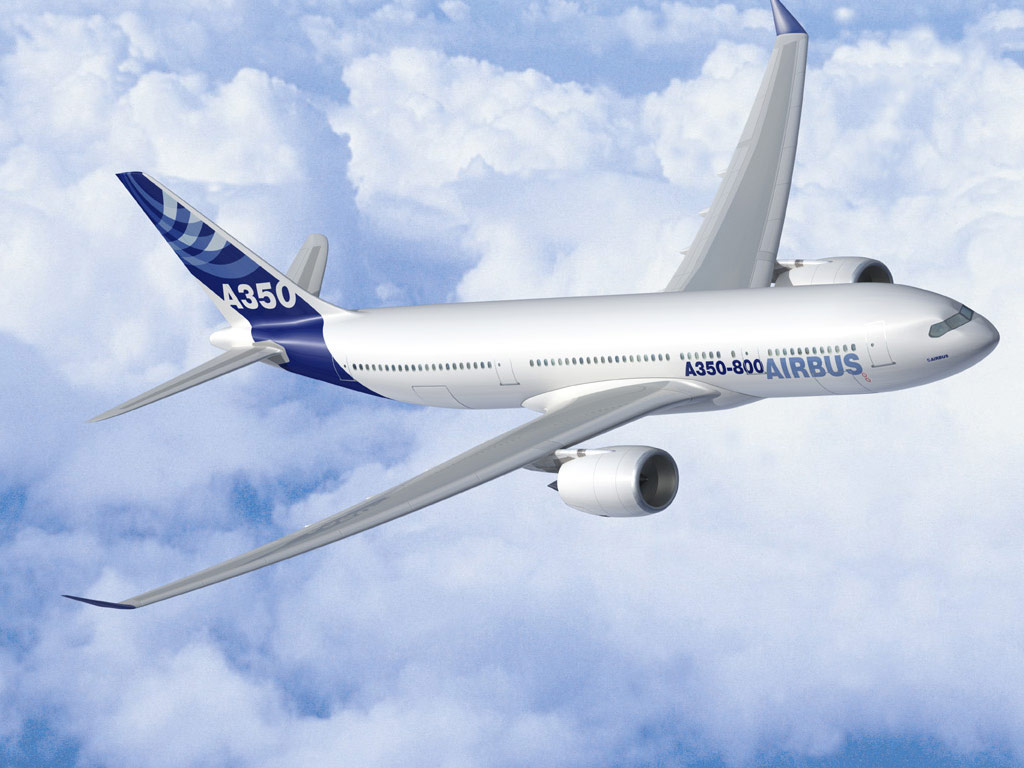
\includegraphics[width=0.25\textwidth]{Figures/Airbus_A350.jpg}
%   \caption[Optional caption for figure in TOC.]{Caption for figure.}
%   \label{fig:airbus1}
% \end{figure}

% It is possible to include subfigures.
% Figure~\ref{fig:aircraft} is composed of three subfigures: Fig.~\ref{fig:aircraft1}, \ref{fig:aircraft2} and \ref{fig:aircraft3}.
% %
% \begin{figure}[!htbp]
%     \centering
%     \subfloat[Airbus A320.\label{fig:aircraft1}]{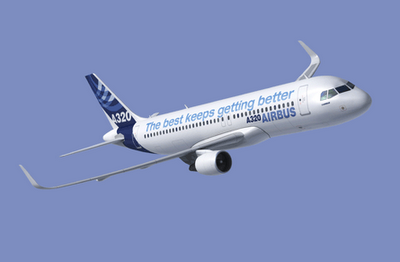
\includegraphics[width=0.49\textwidth]{Figures/Airbus_A320_sharklets.png}]{fig1a}}\hfill
%     \subfloat[Bombardier CRJ200.\label{fig:aircraft2}] {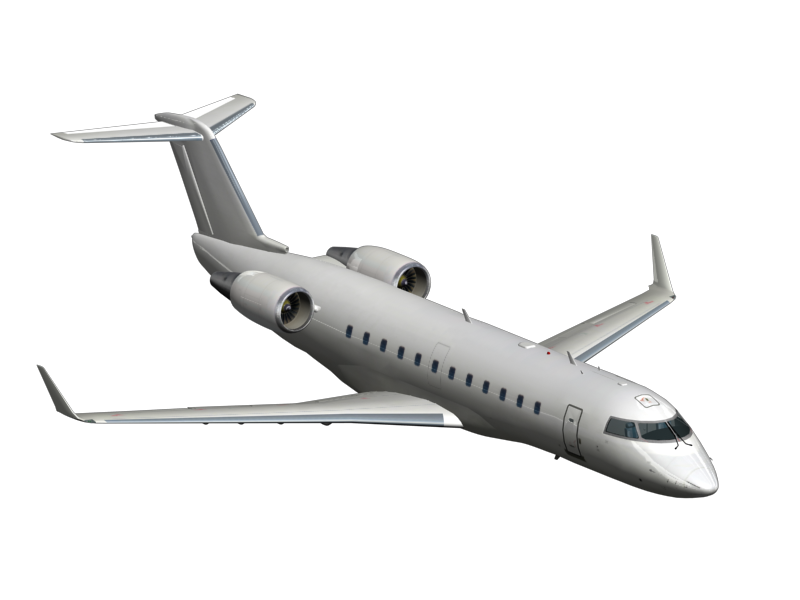
\includegraphics[width=0.49\linewidth]{Figures/Bombardier_CRJ200.png}}\hfill
%     \subfloat[Airbus A350.\label{fig:aircraft3}]{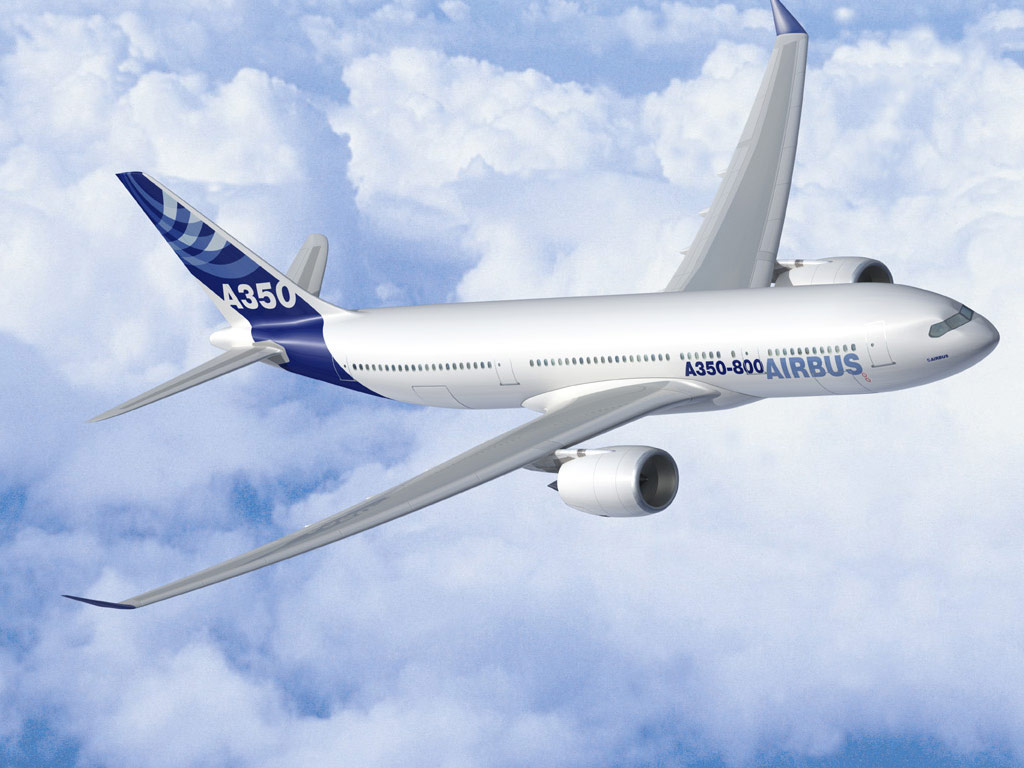
\includegraphics[width=0.49\textwidth]{Figures/Airbus_A350.jpg}}
%     \caption{Examples of aircraft.} \label{fig:aircraft}
% \end{figure}

% Most aircraft have wings with large aspect ratios (\AR = 8 -- 15) for higher aerodynamic efficiency.


% % ----------------------------------------------------------------------
% \subsubsection{Drawings}
% \label{subsection:drawings}

% Insert your subsection material and for instance a few drawings.

% The schematic illustrated in Fig.~\ref{fig:algorithm} can represent some sort of algorithm.

% \begin{figure}[!htb]
%   \centering
%   \scriptsize
% %  \footnotesize 
% %  \small
%   \setlength{\unitlength}{0.9cm}
%   \begin{picture}(8.5,6)
%     \linethickness{0.3mm}

%     \put(3,6){\vector(0,-1){1}}
%     \put(3.5,5.4){$\bf \alpha$}
%     \put(3,4.5){\oval(6,1){}}
%     %\put(0,4){\framebox(6,1){}}
%     \put(0.3,4.4){Grid Generation: \quad ${\bf x} = {\bf x}\left({\bf \alpha}\right)$}

%     \put(3,4){\vector(0,-1){1}}
%     \put(3.5,3.4){$\bf x$}
%     \put(3,2.5){\oval(6,1){}}
%     %\put(0,2){\framebox(6,1){}}
%     \put(0.3,2.4){Flow Solver: \quad ${\cal R}\left({\bf x},{\bf q}\left({\bf x}\right)\right) = 0$}

%     \put(6.0,2.5){\vector(1,0){1}}
%     \put(6.4,3){$Y_1$}

%     \put(3,2){\vector(0,-1){1}}
%     \put(3.5,1.4){$\bf q$}
%     \put(3,0.5){\oval(6,1){}}
%     %\put(0,0){\framebox(6,1){}}
%     \put(0.3,0.4){Structural Solver: \quad ${\cal M}\left({\bf x},{\bf q}\left({\bf x}\right)\right) = 0$}

%     \put(6.0,0.5){\vector(1,0){1}}
%     \put(6.4,1){$Y_2$}

%     %\put(7.8,2.5){\oval(1.6,5){}}
%     \put(7.0,0){\framebox(1.6,5){}}
%     \put(7.1,2.5){Optimizer}
%     \put(7.8,5){\line(0,1){1}}
%     \put(7.8,6){\line(-1,0){4.8}}
%   \end{picture}
%   \caption{Schematic of some algorithm.}
%   \label{fig:algorithm}
% \end{figure}


% % ----------------------------------------------------------------------
% \subsection{Equations}
% \label{subsection:equations}

% Equations can be inserted in different ways.

% The simplest way is in a separate line as

% \begin{equation}
%   \frac{{\rm d} q_{ijk}}{{\rm d} t} + {\cal R}_{ijk}({\bm q}) = 0 \,,
% \label{eq:ode}
% \end{equation}
% %
% where each variable must properly defined.

% If the equation is to be embedded in the text, it can be done like ${\partial {\cal R}}/{\partial {\bm q}}=0$.

% It may also be split in different lines like

% \begin{eqnarray}
%   {\rm Minimize}   && Y({\bm \alpha},{\bm q}({\bm \alpha}))            \nonumber           \\
%   {\rm with~respect~to}     && {\bm \alpha}                                     \label{eq:minimize} \\
%   {\rm subject~to} && {\cal R}({\bm \alpha},{\bm q}({\bm \alpha})) = 0 \nonumber           \\
%                    &&       C ({\bm \alpha},{\bm q}({\bm \alpha})) = 0 \,. \nonumber
% \end{eqnarray}

% It is also possible to use subequations.

% \begin{subequations}
%     \begin{equation}
%     \frac{\partial \rho}{\partial t} + \frac{\partial}{\partial x_j}\left( \rho u_j \right) = 0 \,,
%     \label{eq:continuity}
%     \end{equation}
%     \begin{equation}
%     \frac{\partial}{\partial t}\left( \rho u_i \right) + \frac{\partial}{\partial x_j} \left( \rho u_i u_j + p \delta_{ij} - \tau_{ji} \right) = 0, \quad i=1,2,3 \,,
%     \label{eq:momentum}
%     \end{equation}
%     \begin{equation}
%         \frac{\partial}{\partial t}\left( \rho E \right) + \frac{\partial}{\partial x_j} \left( \rho E u_j + p u_j - u_i \tau_{ij} + q_j \right) = 0 \,.
%     \label{eq:energy}
%     \end{equation}
% \label{eq:NavierStokes}%
% \end{subequations}

% Notice that the equations should be punctuated as they are part of sentences, so a comma or a period should be put at the end of each of them, as exemplified in all the previous equations.

% When referencing an equation, use the abbreviation Eq., unless it is the beginning of a sentence.
% The number of the equation should always be in parenthesis.

% Equations~(\ref{eq:continuity}), (\ref{eq:momentum}) and (\ref{eq:energy}) form the Navier--Stokes equations~(Eq.~ (\ref{eq:NavierStokes})).


% % ----------------------------------------------------------------------
% \subsection{Tables}
% \label{section:tables}

% Insert your subsection material and for instance a few tables.

% Make sure all tables presented are referenced in the text!

% The caption should appear above the table.

% Follow some guidelines when making tables:

% \begin{itemize}
%   \item Avoid vertical lines;
%   \item Avoid “boxing up” cells, usually 3 horizontal lines are enough: above, below, and after heading;
%   \item Avoid double horizontal lines;
%   \item Add enough space between rows.
% \end{itemize}

% \begin{table}[!htb]
%   \caption[Table caption shown in TOC.]{Table caption.}
%   \label{tab:aeroCoeff}
%   \renewcommand{\arraystretch}{1.2} % more space between rows
%   \centering
%   \begin{tabular}{lccc}
%     \toprule
%     Model           & $C_L$ & $C_D$ & $C_{M y}$ \\
%     \midrule
%     Euler           & 0.083 & 0.021 & -0.110    \\
%     Navier--Stokes  & 0.078 & 0.023 & -0.101    \\
%     \bottomrule
%   \end{tabular}
% \end{table}

% When referencing a table, use the abbreviation Tab., unless it is the beginning of a sentence.

% Tables~\ref{tab:memory} and \ref{tab:multipleColumns} are examples of tables with merging columns:

% \begin{table}[!htb]
%   \caption{Memory usage comparison (in MB).}
%   \label{tab:memory}
%   \renewcommand{\arraystretch}{1.2} % more space between rows
%   \centering
%   \begin{tabular}[]{lrr}
%     \toprule
%                 & \multicolumn{2}{c}{\underline{Virtual memory [MB]}} \\
%                 & Euler       & Navier--Stokes \\
%     \midrule
%       Wing only &  1,000      &    2,000       \\
%       Aircraft  &  5,000      &   10,000       \\
%       (ratio)   & $5.0\times$ & $5.0\times$    \\
%     \bottomrule
%   \end{tabular}
% \end{table}

% \begin{table}[!htb]
%   \caption{Another table caption.}
%   \label{tab:multipleColumns}
%   \centering
%   \renewcommand{\arraystretch}{1.2} % more space between rows
%   \begin{tabular}{@{}rrrrcrrr@{}} % remove space to the vertical edges @{}...@{}
%     \toprule
%       & \multicolumn{3}{c}{$w = 2$} & \phantom{abc} & \multicolumn{3}{c}{$w = 4$} \\
%     \cmidrule{2-4}
%     \cmidrule{6-8}
%       & $t=0$ & $t=1$ & $t=2$ && $t=0$ & $t=1$ & $t=2$ \\
%     \midrule
%       $dir=1$
%       \\
%       $c$ &  0.07 &  0.16 &  0.29 &&  0.36 &  0.71 &   3.18 \\
%       $c$ & -0.86 & 50.04 &  5.93 && -9.07 & 29.09 &  46.21 \\
%       $c$ & 14.27 &-50.96 &-14.27 && 12.22 &-63.54 &-381.09 \\
%       $dir=0$
%       \\
%       $c$ &  0.03 &  1.24 &  0.21 &&  0.35 & -0.27 &  2.14 \\
%       $c$ &-17.90 &-37.11 &  8.85 &&-30.73 & -9.59 & -3.00 \\
%       $c$ &105.55 & 23.11 &-94.73 &&100.24 & 41.27 &-25.73 \\
%     \bottomrule
%   \end{tabular}
% \end{table}

% An example with merging rows can be seen in Tab.~\ref{tab:multipleRows}.

% \begin{table}[!htb]
%   \caption{Yet another table caption.}
%   \label{tab:multipleRows}
%   \renewcommand{\arraystretch}{1.2} % more space between rows
%   \centering
%   \begin{tabular}{ccccc}
%     \toprule
%       \multirow{2}{*}{ABC} & \multicolumn{4}{c}{header} \\
%       \cmidrule{2-5} & 1.1 & 2.2 & 3.3 & 4.4 \\
%     \midrule
%       \multirow{2}{*}{IJK} & \multicolumn{2}{c}{\multirow{2}{*}{group}} & 0.5 & 0.6 \\
%       \cmidrule{4-5}       & \multicolumn{2}{c}{}                       & 0.7 & 1.2 \\
%     \bottomrule
%   \end{tabular}
% \end{table}

% If a table has too many columns, it can be scaled to fit the text width, as in Tab.~\ref{tab:scale}.
% %
% \begin{table}[!htb]
%   \caption{Very wide table.}
%   \label{tab:scale}%
%   \renewcommand{\arraystretch}{1.2} % more space between rows
%   \centering
%   \resizebox*{\textwidth}{!}{%
%     \begin{tabular}[]{lcccccccccc}
%       \toprule
%         Variable &  a  &  b  &  c  &  d  &  e  &  f  &  g  &  h  &  i  &  j  \\
%       \midrule
%         Test 1   &  10,000 &  20,000 &  30,000 &  40,000 &  50,000 &  60,000 &  70,000 &  80,000 &  90,000 & 100,000 \\
%         Test 2   &  20,000 &  40,000 &  60,000 &  80,000 & 100,000 & 120,000 & 140,000 & 160,000 & 180,000 & 200,000 \\
%       \bottomrule
%     \end{tabular}
%   }%
% \end{table}


% % ----------------------------------------------------------------------
% \subsection{Mixing}
% \label{section:mixing}

% If necessary, a figure and a table can be put side-by-side as in Fig.~\ref{fig:side_by_side}

% \begin{figure}[!htb]
%   \begin{minipage}[b]{0.60\linewidth}
%     \centering
%     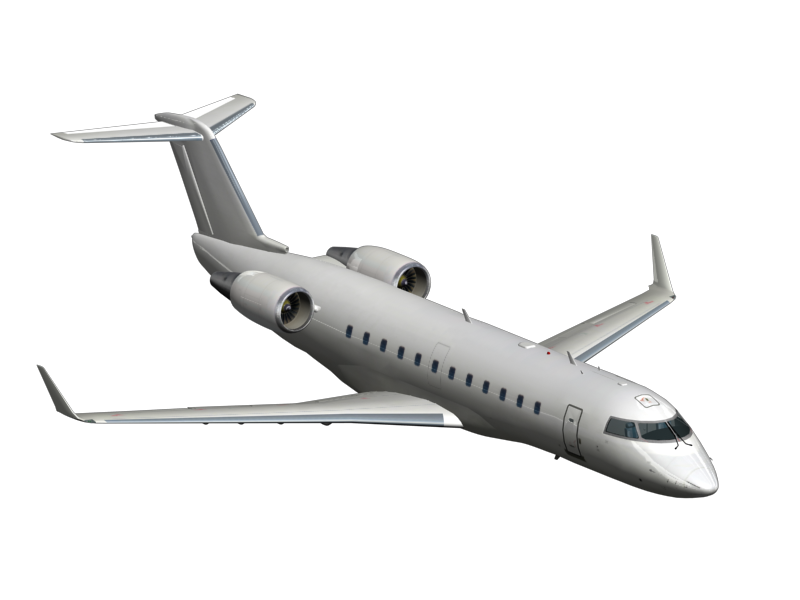
\includegraphics[width=\linewidth]{Figures/Bombardier_CRJ200}
%   \end{minipage}%
%   \begin{minipage}[b]{0.30\linewidth}
%     \centering
%     \begin{tabular}[b]{lll}
%       \toprule
%         \multicolumn{3}{c}{Legend} \\
%       \midrule
%         A & B & C \\
%         0 & 0 & 0 \\
%         0 & 1 & 0 \\
%         1 & 0 & 0 \\
%         1 & 1 & 1 \\
%       \bottomrule
%     \end{tabular}
%     \vspace{5em}
%   \end{minipage}
% \caption{Figure and table side-by-side.}
% \label{fig:side_by_side}
% \end{figure}

